\documentclass[conference]{IEEEtran}

\usepackage{cite}
\usepackage{graphicx}
\usepackage{amsmath,amssymb}
\usepackage{booktabs}
\usepackage{array}
\usepackage{multirow}
\usepackage{url}
\usepackage{algorithm}
\usepackage{algpseudocode}
\usepackage{placeins}
\usepackage{xcolor}

\graphicspath{{figures/}}

\begin{document}

\title{A Machine Learning-Driven Stray Animal Welfare Intelligence Framework for Bangladesh}

\author{
\IEEEauthorblockN{Sazzad Kazi, Iqra Siddique}
\IEEEauthorblockA{
Data Science Program\\
Department of Computer Science and Engineering\\
United International University\\
Dhaka, Bangladesh
}
}

\maketitle

\begin{abstract}
Stray animal welfare in Bangladesh is closely connected with public health,
human--animal conflict, disease prevention, and humane urban animal
management. However, relevant information is fragmented across online news
reports and localized field observations, limiting the ability to obtain
structured and actionable welfare intelligence. This study presents a
machine learning-driven, dual-source stray animal welfare intelligence
framework for Bangladesh that integrates Bangladesh-focused online news
analysis with a pilot field survey conducted in Badda, Dhaka.

The news intelligence pipeline initially collected 1,094 records and applied
relevance filtering, geographic scope refinement, weak labeling, and
assisted review. This process produced a final machine learning corpus of
226 Bangladesh-focused records. TF--IDF text representations were evaluated
using Linear Support Vector Machine (SVM), Logistic Regression, and
Complement Naive Bayes classifiers. Linear SVM achieved the best overall
performance, with a macro F1-score of 0.6068 and a weighted F1-score of
0.7517. An interpretable Stray Abuse Risk Index (SARI V2) was additionally
used as a separate heuristic assessment mechanism, producing a mean score
of 1.550 and a maximum score of 5.500.

To complement media-derived intelligence with ground-level evidence, a
structured pilot survey of 325 stray animals was conducted across selected
areas of Badda, Dhaka. The survey recorded animal type, age, observed health
condition, vaccination status, sterilization status, behavior, and location.
Within the surveyed sample, 9.85\% of animals were reported as vaccinated,
10.46\% as sterilized, and 28.62\% showed observed nutritional health
concerns. The field survey is treated as a localized case study rather than
a nationally representative prevalence estimate.

By combining broader Bangladesh-focused incident intelligence with localized
field observations, the proposed framework demonstrates a scalable approach
for transforming heterogeneous animal-welfare information into structured
evidence. The framework may support future data-driven vaccination,
sterilization, welfare monitoring, and intervention planning while providing
a foundation for expansion to additional areas of Bangladesh.
\end{abstract}

\begin{IEEEkeywords}
stray animal welfare, machine learning, natural language processing,
human--animal conflict, rabies, SARI, field survey, Bangladesh,
One Health, decision support
\end{IEEEkeywords}

\section{Introduction}

Free-roaming dogs and cats are a visible component of urban environments in
Bangladesh, where animal welfare, public health, community safety, and human
behavior are closely interconnected. Stray animals may experience food
scarcity, malnutrition, disease, injury, abuse, poisoning, and inadequate
access to veterinary care. At the same time, concerns regarding dog bites,
rabies transmission, aggressive behavior, and unmanaged animal populations
can contribute to negative human--animal interactions. Consequently, the
management of free-roaming animals is not solely an animal-welfare issue; it
also represents a public-health and community-management challenge.

Rabies provides a particularly important example of this relationship.
Bangladesh has implemented large-scale dog vaccination and rabies-control
programs, demonstrating the importance of coordinated interventions involving
human health, animal health, and local communities. Such challenges are
consistent with the One Health perspective, in which human, animal, and
environmental health are considered interconnected. Nevertheless, vaccination
and disease control represent only part of the broader stray-animal welfare
problem. Abuse, killing, poisoning, rescue events, nutritional condition,
sterilization coverage, and human--animal conflict also require systematic
monitoring.

A major challenge is the fragmentation of relevant information. Reports of
animal abuse, rabies concerns, dog bites, rescue operations, poisoning, and
other welfare-related events are distributed across numerous online news
sources. These reports are primarily unstructured text and are therefore
difficult to analyze systematically at scale. Field-level information creates
a second challenge. Variables such as visible health condition, vaccination,
sterilization, age, and animal behavior are generally unavailable from news
reports alone. Consequently, relying on either media reports or localized
field observations in isolation provides only a partial view of the problem.

An earlier version of this research established a news-based analytical
framework for Bangladesh in which online reports were collected, processed,
categorized using rule-based techniques, and evaluated using a custom Stray
Abuse Risk Index (SARI). Although the framework demonstrated the feasibility
of transforming dispersed news reports into structured incident information,
several limitations remained. Classification depended primarily on
keyword-based rules, many headlines contained insufficient contextual
information, geographic information was inconsistent, and the system lacked
direct field-level observations of stray-animal welfare conditions.

The present study extends that foundation by introducing a machine
learning-driven dual-source welfare intelligence framework. The first
component, termed \textit{News Intelligence}, collects and refines
Bangladesh-focused news records and applies natural language processing and
supervised text classification to identify incident categories. The second
component, termed \textit{Field Intelligence}, incorporates structured
ground-level observations collected through a pilot survey in Badda, Dhaka.
Rather than merging these heterogeneous datasets at the individual-record
level, the framework treats them as complementary evidence streams.

The news-processing pipeline was designed with multiple refinement stages.
A total of 1,094 news records were initially assembled. Relevance filtering
retained 690 records, after which geographic scope filtering identified 250
Bangladesh-primary records. Assisted review and corpus preparation produced a
final set of 226 records for machine-learning experiments. Three traditional
text classifiers---Linear Support Vector Machine (SVM), Logistic Regression,
and Complement Naive Bayes---were evaluated using TF--IDF representations.
Linear SVM achieved the highest macro F1-score among the evaluated models.

A revised SARI mechanism, referred to as SARI V2, was maintained separately
from the machine-learning classification target. Instead of training a model
to reproduce a risk label generated from deterministic rules, SARI V2 serves
as an interpretable heuristic index based on textual indicators associated
with abuse, human conflict, sickness or rabies, poisoning, and contextual
incident severity. This separation reduces circularity between incident
classification and risk assessment while preserving interpretability.

To introduce direct field evidence, 325 stray animals were surveyed in four
localities within Badda, Dhaka: Uttar Badda, Dokkhin Badda, Moddho Badda, and
Jheelpar. The survey captured information on animal type, age, approximate
weight, observed health condition, visible health issues, vaccination,
sterilization, behavior, and location. Badda is used as a pilot case-study
area for demonstrating the field-intelligence component of the proposed
framework. The observations are therefore not interpreted as nationally
representative estimates of stray-animal conditions in Bangladesh.

The main contributions of this study are summarized as follows:
\begin{itemize}
    \item A Bangladesh-focused, dual-source stray-animal welfare intelligence
    framework integrating online news analysis with localized field evidence.
    
    \item A multi-stage data-refinement pipeline that reduces a heterogeneous
    collection of 1,094 news records to a more focused 226-record corpus for
    incident-classification experiments.
    
    \item A comparative evaluation of Linear SVM, Logistic Regression, and
    Complement Naive Bayes using TF--IDF text features and class-sensitive
    evaluation metrics.
    
    \item An interpretable SARI V2 mechanism maintained separately from the
    supervised incident-classification target.
    
    \item A structured pilot field survey of 325 stray animals in Badda,
    Dhaka, providing localized evidence regarding observed health,
    vaccination, sterilization, behavior, and spatial variation.
    
    \item An evidence-level integration strategy that combines media-derived
    incident intelligence and field observations without incorrectly treating
    the two heterogeneous datasets as directly interchangeable samples.
\end{itemize}

The resulting framework is intended as a scalable analytical foundation rather
than a complete national surveillance system. By extending field data
collection to additional areas and improving the quality and coverage of
textual incident data, the proposed approach can support broader animal-welfare
monitoring and intervention planning in Bangladesh.

% =========================================================
% II. LITERATURE REVIEW AND STATE OF THE ART
% =========================================================

\section{Literature Review and State of the Art}

\subsection{Stray Animal Management and Rabies in Bangladesh}

Free-roaming animal management in Bangladesh has historically been closely
associated with rabies prevention and public-health interventions. Rabies is
a vaccine-preventable zoonotic disease, and dogs are the principal source of
human rabies transmission in endemic settings. Consequently, dog vaccination,
population management, bite prevention, and access to post-exposure
prophylaxis are central components of rabies-control strategies
\cite{who_rabies_bd}.

Bangladesh has progressively adopted a One Health-oriented approach to rabies
control. The national strategy has included mass dog vaccination (MDV),
post-exposure prophylaxis for bite victims, public awareness, and
multisectoral coordination. According to the World Health Organization,
approximately 1.7 million dogs live in Bangladesh, with a large proportion
free-roaming. Bangladesh expanded its mass dog vaccination activities from
an initial pilot intervention into a broader national programme
\cite{who_mdv_2022}.

Tenzin et al. conducted an important field-based investigation of
free-roaming dogs in Dhaka City \cite{tenzin2015}. Using surveys across
sampled city wards, the study estimated the free-roaming dog population and
evaluated the progress of a Catch-Neuter-Vaccinate-Release (CNVR) programme.
The work demonstrated the importance of localized field observation for
understanding animal populations and evaluating vaccination and sterilization
interventions. However, its primary objective was population estimation and
rabies-control programme assessment rather than automated analysis of
animal-welfare incidents from heterogeneous information sources.

More recently, Ghosh et al. analyzed Bangladesh's rabies-control programme
using data spanning 2011--2023 \cite{ghosh2024}. Their One Health study
integrated multiple epidemiological and vaccination-related data sources and
reported an estimated national dog population of approximately 1.67 million.
The analysis indicated that expansion of mass dog vaccination and human
anti-rabies vaccination was associated with substantial progress in rabies
control. Such findings demonstrate the value of combining multiple data
sources for animal and public-health decision making.

Recent field evidence further demonstrates the importance of localized
vaccination monitoring in Bangladesh. Swedberg et al. evaluated mass dog
vaccination strategies across four urban and peri-urban study sites and
reported that 9,195 dogs were vaccinated during the evaluated campaigns
\cite{swedberg2026}. Post-vaccination surveys indicated that more than 93\%
of observed dogs were free-roaming, while estimated vaccination coverage
varied substantially depending on both the vaccination strategy and the
enumeration method. The study highlights the practical importance of
location-specific monitoring and reliable field-survey methods rather than
relying on a single national population assumption.

These studies establish a strong foundation for rabies surveillance and dog
population management in Bangladesh. Nevertheless, rabies represents only one
dimension of stray-animal welfare. Abuse, killing, poisoning, rescue events,
nutritional condition, visible health problems, sterilization status, and
human--animal conflict require broader analytical approaches.

\subsection{News-Based Event Intelligence and Text Classification}

Online news platforms provide a continuously growing source of unstructured
information about social and public-health events. News reports can contain
information regarding animal abuse, poisoning, killing, rescue operations,
rabies concerns, bite incidents, community responses, and animal-management
activities. However, manually reviewing large numbers of reports is
time-consuming and makes systematic monitoring difficult.

Natural language processing (NLP) and machine-learning techniques provide a
mechanism for transforming such unstructured text into structured event
categories. In a conventional text-classification pipeline, textual documents
are first converted into numerical representations before being supplied to a
classifier. Term Frequency--Inverse Document Frequency (TF--IDF) remains a
widely used representation for text retrieval and classification because it
emphasizes terms that are informative within a document while reducing the
influence of terms that occur frequently across the corpus
\cite{salton1988}.

Linear classifiers are particularly suitable for sparse, high-dimensional
text representations. Support Vector Machines have been widely studied for
such classification problems \cite{cortes1995}, and Joachims demonstrated
their effectiveness specifically for text categorization with many relevant
features \cite{joachims1998}. Complement Naive Bayes provides another useful
approach for addressing limitations of conventional Naive Bayes assumptions
in text classification \cite{rennie2003}. Accordingly, the present study
evaluates Linear SVM, Logistic Regression, and Complement Naive Bayes using
the same refined news corpus rather than assuming that a more computationally
complex model will necessarily perform better.

Model evaluation also requires more than overall accuracy when the class
distribution is imbalanced. Macro-averaged precision, recall, and F1 score
provide a useful view of performance because each class contributes equally
to the macro average, including classes with relatively few observations
\cite{sokolova2009}. The machine-learning pipeline was implemented using
Scikit-learn \cite{pedregosa2011}. In addition to predictive performance,
feature-level inspection was used to examine which textual terms contributed
most strongly to individual class decisions, following the broader importance
of feature analysis in text-classification systems \cite{forman2003}.

\subsection{Weak Supervision and Assisted Label Construction}

A major limitation in domain-specific text classification is the cost of
constructing a sufficiently large manually annotated training dataset.
Weak-supervision approaches address this problem by using heuristics, rules,
existing knowledge, or other imperfect sources to generate candidate labels.

Ratner et al. introduced Snorkel as a framework for creating training data
from user-defined labeling functions instead of relying exclusively on
manually labeled examples \cite{ratner2017}. Their work demonstrates the
broader principle that imperfect programmatic supervision can be useful when
large manually labeled datasets are unavailable.

The labeling procedure in the present study is inspired by this general
weak-supervision principle but does not implement the Snorkel system.
Candidate incident labels are first generated through domain-specific textual
rules. A stratified validation sample is subsequently inspected through an
assisted review process to identify obvious out-of-scope records, ambiguous
cases, and incorrect suggested labels. The resulting labels should therefore
be interpreted as weakly supervised and partially reviewed labels rather than
as a fully independent expert-annotated gold-standard corpus.

This distinction is particularly important when interpreting classifier
performance. Cross-validation scores in this study measure predictive
agreement with the constructed labels and should not be interpreted as an
independent estimate of expert-level classification accuracy.

\subsection{Field-Based Welfare Observation}

Reliable management of free-roaming animal populations also depends on
appropriate field-observation and population-estimation methods. Belo et al.
systematically reviewed approaches used to estimate free-ranging dog
populations and emphasized the importance of understanding population
structure and abundance for the planning and monitoring of population-control
and animal-welfare interventions \cite{belo2015}. This broader methodological
perspective supports the use of localized field evidence alongside
event-oriented information sources.

Evidence from dog population management research also shows that intervention
effectiveness cannot be assessed using population size alone. Smith et al.
systematically reviewed dog population management studies across multiple
countries and found that programmes have been evaluated using outcomes related
to population size, dog health and welfare, public-health risk, and community
attitudes \cite{smith2019dpm}. Their review also identified substantial
variation in study design and reporting quality, reinforcing the need for
clearly defined indicators when evaluating vaccination, sterilization, and
other management interventions.

More recent experimental evidence also shows why intervention outcomes should
be evaluated rather than assumed. Fielding et al. conducted a multi-site
randomised controlled trial of intensive surgical sterilisation in
free-roaming dog populations \cite{fielding2025sterilisation}. Female
sterilisation coverage reached approximately 58--66\% in intervention areas.
Although reductions were observed in puppies, lactating females, and some
reported nuisance behaviours, the study did not find a significant reduction
in adult free-roaming dog counts during the two-year follow-up. These findings
illustrate that sterilisation outcomes can depend on population movement,
coverage, and local conditions, reinforcing the need for location-specific
monitoring alongside intervention delivery.

News-derived information provides evidence regarding events that receive
media coverage, but it cannot reliably describe the everyday welfare
condition of individual free-roaming animals. Variables such as observed
nutritional condition, approximate age, vaccination status, sterilization
status, visible health problems, and behavior generally require direct
field-level observation.

Localized animal surveys therefore provide a complementary evidence source.
In Dhaka, Tenzin et al. used direct field observation not only to estimate
free-roaming dog populations and CNVR coverage but also to record observable
characteristics including approximate age, body condition, skin condition,
and sterilization and vaccination status \cite{tenzin2015}. Their findings
illustrate how structured field observations can provide information that is
not normally available from event-oriented news reports.

Building on this field-based perspective, the present study incorporates a
structured survey of 325 observed animals from four localities in Badda,
Dhaka. The survey records variables related to animal type, approximate age,
observed nutritional condition, vaccination status, sterilization status,
behavior, visible health concerns, and location. Unlike a national prevalence
survey, this component is treated as a localized pilot case study. Its purpose
is to demonstrate how field-level welfare observations can complement the
Bangladesh-focused news intelligence pipeline without implying that the Badda
sample represents the national stray-animal population.

\subsection{Need for Multi-Source Welfare Intelligence}

International guidance increasingly treats free-roaming dog management as a
multisectoral problem involving animal welfare, public health, population
management, community behavior, and disease prevention. The World Organisation
for Animal Health (WOAH) recommends a holistic dog population management
approach that improves dog health and welfare while addressing public-health
and safety concerns. Importantly, such programmes should consider local dog
population dynamics and community conditions rather than applying identical
interventions across different settings \cite{woah_dpm2024}.

This perspective is consistent with the broader One Health framework. The
global ``Zero by 30'' strategy emphasizes coordinated surveillance, mass dog
vaccination, community engagement, and access to human post-exposure
prophylaxis for eliminating dog-mediated human rabies deaths
\cite{who_zero2030}. More broadly, the Quadripartite One Health Joint Plan of
Action promotes collaboration across human, animal, and environmental health
systems for monitoring and responding to interconnected health risks
\cite{onehealth2022}. These principles support the development of analytical
systems that combine multiple forms of evidence rather than treating animal
welfare and public-health observations as isolated problems.

Existing Bangladesh-focused research provides valuable evidence regarding
rabies epidemiology, vaccination, and free-roaming dog population management.
However, these objectives differ from the problem of building an integrated
animal-welfare intelligence system.

A broader system should be capable of examining both reported incidents and
ground-level welfare indicators. News reports provide one perspective by
capturing socially visible incidents, whereas field surveys provide another
by documenting observed animal conditions within a defined locality. These
sources have different units of observation and sampling mechanisms and
therefore should not be directly merged as if they represented a single
homogeneous dataset.

The present study addresses this issue through a dual-source architecture.
Bangladesh-focused news records are processed through an NLP and
machine-learning pipeline to create incident intelligence, while the Badda
pilot survey provides localized field intelligence. The two components are
integrated at the evidence and decision-support level rather than through
row-level data fusion.

Recent evidence also highlights continuing methodological gaps in the
monitoring of free-roaming dog populations. A scoping review by Cunha Silva
et al. found substantial variation in dog-enumeration and movement-study
methods across rabies-endemic settings and identified important gaps in the
evidence needed for effective intervention planning
\cite{cunhasilva2025}. These limitations further support the use of clearly
defined, location-aware indicators when developing welfare and
public-health decision-support systems.

% =========================================================
% III. RESEARCH GAP AND CONTRIBUTIONS
% =========================================================

\section{Research Gap and Contributions}

Despite substantial progress in rabies control and free-roaming dog
management, several gaps remain in the development of data-driven
stray-animal welfare intelligence for Bangladesh.

First, much of the existing Bangladesh-focused literature emphasizes rabies,
dog population estimation, vaccination, and disease prevention. These are
essential public-health objectives, but they do not provide a unified
mechanism for monitoring heterogeneous welfare-related incidents such as
abuse, killing, poisoning, rescue, disease-related events, and
human--animal conflict.

Second, animal-welfare information reported by online media remains
unstructured and distributed across multiple sources. A simple keyword-based
system can provide an initial analytical solution but has limited ability to
generalize across linguistic variations and contextual expressions. This
motivates the transition from purely rule-based incident assignment toward
supervised text classification.

Third, the absence of a large expert-annotated Bangladesh-specific
stray-animal incident corpus creates a training-data challenge. The present
study therefore investigates a weak-supervision-inspired labeling strategy
combined with assisted review while explicitly acknowledging that the
resulting corpus is not equivalent to independently annotated ground truth.

Fourth, news reports alone cannot provide sufficient information regarding
the routine condition of free-roaming animals. Media coverage is event-driven
and may preferentially represent unusual, controversial, or severe incidents.
Direct field observations are therefore necessary to provide complementary
information regarding health condition, vaccination, sterilization, age, and
behavior.

Finally, localized field observations cannot automatically be generalized to
the entire country. A framework is needed that can preserve the distinction
between broader Bangladesh-focused incident intelligence and localized
ground-level evidence while still allowing both to contribute to
decision-support.

To address these gaps, this study makes four principal methodological
advances over the earlier framework:

\begin{enumerate}
    \item It replaces exclusive dependence on rule-based incident
    classification with a comparative machine-learning experiment using
    TF--IDF features and three supervised text classifiers.

    \item It introduces a multi-stage relevance and geographic-scope
    refinement process to construct a more focused Bangladesh-primary news
    corpus.

    \item It separates incident prediction from the SARI V2 heuristic risk
    assessment, avoiding the use of deterministic risk labels as a supervised
    machine-learning target.

    \item It extends the framework beyond media intelligence by incorporating
    a 325-animal pilot field survey in Badda, Dhaka, while preserving the
    localized nature of the survey findings.
\end{enumerate}

Together, these contributions transform the earlier news-based analytical
pipeline into a dual-source welfare intelligence framework that combines
machine-learning-based incident analysis with structured field evidence.% =========================================================


% =========================================================
% IV. DATASET CONSTRUCTION AND DATA REFINEMENT
% =========================================================

\section{Dataset Construction and Data Refinement}

The proposed framework relies on two fundamentally different sources of
evidence. The first is a collection of online news records used to study
reported stray-animal incidents in the Bangladesh context. The second is a
structured field survey designed to observe the condition of free-roaming
animals within a selected pilot area in Badda, Dhaka. These datasets were
kept separate throughout preprocessing and analysis because they represent
different units of observation: a news record describes a reported event,
whereas a survey record represents an observed animal.

\subsection{News Data Collection}

The news component was developed by expanding the data-collection process
used in the earlier version of the project. Google News RSS was used as the
primary discovery mechanism, with search queries covering topics such as
stray dogs and cats, animal abuse, killing, poisoning, rescue, dog bites,
rabies, vaccination, disease, and human--animal conflict. Bangladesh-related
terms and selected location-oriented queries were also used to improve the
coverage of locally relevant reports.

For each retrieved item, the pipeline retained the available headline,
source, publication date, link, search context, and RSS description when
present. RSS descriptions were useful because headlines alone frequently
contained insufficient context for distinguishing between superficially
similar incidents.

After combining newly retrieved records with the earlier collection and
removing duplicate entries, the expanded dataset contained 1,094 unique news
records. Publication dates were successfully parsed for all 1,094 records,
and the collection represented 260 unique news sources. Usable RSS
descriptions were available for 387 records. The remaining records therefore
depended more heavily on information available in their headlines.

This expanded collection was intentionally treated as a broad candidate pool
rather than as the final Bangladesh incident dataset. Search-engine retrieval
can return records that contain relevant keywords while describing unrelated,
foreign, wildlife-related, or otherwise out-of-scope events. Consequently,
several refinement stages were applied before the data were used for
machine-learning experiments.

\subsection{Content-Based Relevance Filtering}

The first refinement stage evaluated whether a retrieved record actually
contained evidence of a stray-animal or closely related welfare event.
Importantly, relevance was determined from the available title and RSS
description rather than from the search query that retrieved the article.
This distinction reduced the possibility of retaining a record simply because
a relevant phrase had been used during retrieval.

The relevance rules considered textual evidence associated with dogs, cats,
stray or free-roaming animals, rabies, animal attacks, abuse, poisoning,
killing, rescue, vaccination, disease, and related welfare or conflict
concepts. Records without sufficient evidence were moved to a separate
rejected collection rather than silently discarded.

From the initial 1,094 records, 690 were retained after content-based
relevance filtering, corresponding to a retention rate of approximately
63.1\%. A total of 404 records were rejected at this stage. Among the 690
retained records, 256 contained usable RSS descriptions. Dog-related records
formed the largest animal category, followed by records in which the animal
could not be confidently identified from the available text.

\subsection{Bangladesh Scope Refinement}

Relevance to stray animals does not necessarily imply relevance to
Bangladesh. The initial relevance-filtered corpus still contained reports
from other countries as well as records whose geographic relationship with
Bangladesh was uncertain. A second filtering stage was therefore introduced
to separate the data according to geographic and topical scope.

Geographic evidence was inferred from explicit references to Bangladesh,
recognized Bangladeshi locations, and a curated set of Bangladesh-based news
sources. The search query itself was deliberately excluded as evidence of
geographic origin because a Bangladesh-oriented query can still retrieve a
foreign event.

The scope-refinement procedure separated the 690 relevant records into three
groups:

\begin{itemize}
    \item \textbf{Bangladesh-primary}: records with sufficient evidence that
    the event or reporting context was relevant to Bangladesh;
    
    \item \textbf{Foreign/background}: relevant animal-welfare records that
    could provide contextual information but did not describe a
    Bangladesh-primary event; and
    
    \item \textbf{Out-of-scope}: records dominated by wildlife, unrelated
    meanings, or other content unsuitable for the target incident corpus.
\end{itemize}

This procedure produced 250 Bangladesh-primary records, 331
foreign/background records, and 109 out-of-scope records. Thus, only 36.2\%
of the 690 relevance-filtered records were retained as Bangladesh-primary
evidence. This reduction illustrates why keyword retrieval alone was
insufficient for constructing the final analytical corpus.

Among the 250 Bangladesh-primary records, 175 contained explicit
Bangladesh or local-place evidence, while another 75 were retained through
evidence associated with Bangladesh-based sources. The records covered the
period from 2011 to 2026 and represented 48 unique primary news sources.

\begin{table}[!t]
\centering
\caption{News Dataset Refinement Stages}
\label{tab:data_refinement}
\renewcommand{\arraystretch}{1.15}
\begin{tabular}{lrr}
\toprule
\textbf{Stage} & \textbf{Records} & \textbf{Retained} \\
\midrule
Expanded candidate collection & 1,094 & 100.0\% \\
Content-relevant records       & 690   & 63.1\% \\
Bangladesh-primary records     & 250   & 22.9\% \\
Final ML corpus                & 226   & 20.7\% \\
\bottomrule
\end{tabular}
\end{table}

Figure~\ref{fig:data_funnel} summarizes the complete refinement process.

\begin{figure}[!t]
    \centering
    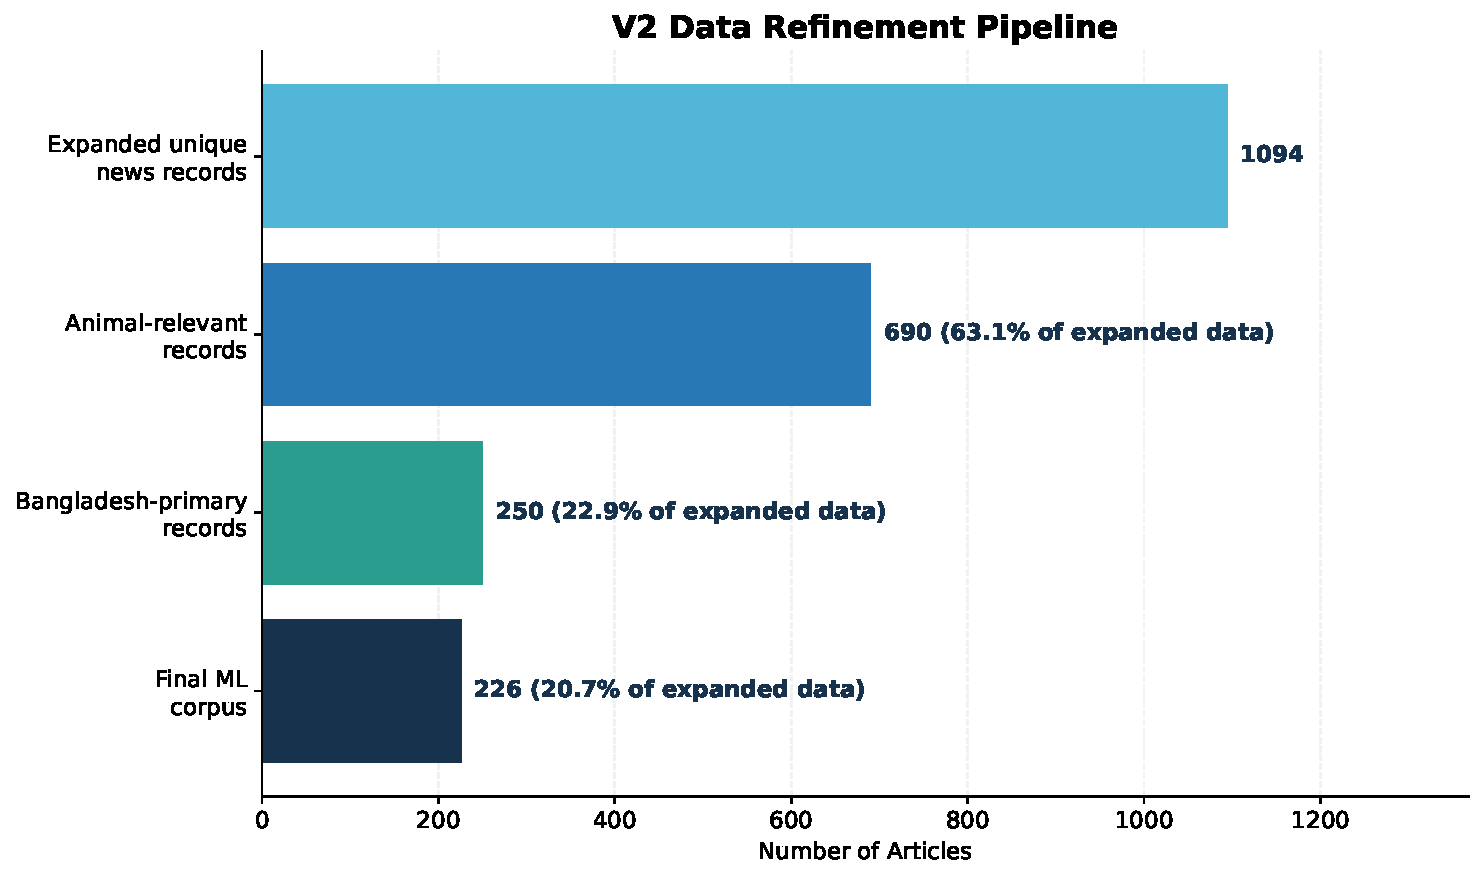
\includegraphics[width=\columnwidth]
    {final_data_refinement_funnel.pdf}
    \caption{Refinement of the news corpus from the expanded candidate
    collection to the final machine-learning dataset.}
    \label{fig:data_funnel}
\end{figure}

\subsection{Initial Incident Label Construction}

The Bangladesh-primary corpus did not contain manually supplied incident
labels. Initial labels were therefore generated using a
weak-supervision-inspired rule system based on textual indicators in the
available headline and description.

Eight incident categories were considered:
\textit{Abuse}, \textit{Conflict}, \textit{Disease},
\textit{Human-Animal Conflict}, \textit{Killing}, \textit{Other},
\textit{Poisoning}, and \textit{Rescue}. These categories were selected to
represent both direct animal-welfare incidents and broader events relevant
to interactions between free-roaming animals and human communities.

The initial labeling process assigned the 250 Bangladesh-primary records as
follows: 99 Other, 39 Disease, 35 Killing, 28 Conflict, 26 Abuse,
13 Human-Animal Conflict, 7 Rescue, and 3 Poisoning. The strong imbalance
between categories was retained rather than artificially balancing the
dataset through synthetic observations, because the objective was to preserve
the characteristics of the collected corpus.

\subsection{Assisted Review and Corpus Finalization}

Programmatically generated labels are imperfect. A stratified validation
sample of 64 records was therefore constructed to inspect the behavior of the
labeling procedure across incident categories. Each sampled record was
examined using its available title and description and assigned one of three
review decisions: \textit{Keep}, \textit{Exclude}, or \textit{Ambiguous}.

The review retained 40 records, excluded 22, and marked 2 as ambiguous.
Examples of excluded content included wildlife-related events, foreign
incidents, unrelated uses of animal terminology, political expressions such
as ``dog whistle,'' and records that did not describe a relevant incident.
Among the 40 retained records, the initial suggested label agreed with the
assisted-review label in 90.0\% of cases.

This 90.0\% agreement should not be interpreted as classifier accuracy.
It measures agreement between the programmatically suggested labels and the
assisted review for the subset of records that were retained. Furthermore,
the complete corpus was not independently annotated by multiple domain
experts. The labels used for machine learning are therefore described
throughout this paper as weakly supervised and partially reviewed rather
than as a gold-standard annotation set.

After removing reviewed exclusions and ambiguous cases from the
Bangladesh-primary collection, 226 records remained in the final
machine-learning corpus.

\begin{table}[!t]
\centering
\caption{Final Machine-Learning Corpus by Incident Category}
\label{tab:final_classes}
\renewcommand{\arraystretch}{1.15}
\begin{tabular}{lr}
\toprule
\textbf{Incident Category} & \textbf{Records} \\
\midrule
Other                     & 90 \\
Disease                   & 39 \\
Killing                   & 31 \\
Conflict                  & 29 \\
Abuse                     & 21 \\
Human-Animal Conflict     & 11 \\
Poisoning                 & 3 \\
Rescue                    & 2 \\
\midrule
\textbf{Total}            & \textbf{226} \\
\bottomrule
\end{tabular}
\end{table}

The final distribution is highly imbalanced. In particular, Poisoning and
Rescue contain only three and two records, respectively. This characteristic
has direct implications for model evaluation: performance estimates for the
rarest classes are inherently unstable, and overall accuracy alone would
provide an incomplete description of classifier behavior.

\subsection{Pilot Field Survey Dataset}

The second evidence stream was constructed independently from the news
corpus. A structured field survey recorded 325 free-roaming animals across
four localities in Badda, Dhaka: Uttar Badda, Dokkhin Badda, Moddho Badda,
and Jheelpar.

The survey was designed to capture variables that cannot normally be inferred
reliably from news reports. These included animal type, estimated age group,
approximate weight, observed nutritional or general health condition,
visible health issues, vaccination status, sterilization status, behavior
toward humans, and the location in which the animal was observed.

Of the 325 observed animals, 322 were dogs and 3 were cats. The largest
geographic share came from Uttar Badda with 219 observations, followed by
Dokkhin Badda with 43, Moddho Badda with 39, and Jheelpar with 24.

Survey responses contained several free-text and inconsistent fields,
particularly approximate weight and visible health issues. Weight entries
included exact values, ranges, upper or lower bounds, textual descriptions,
and values written using different formatting conventions. These entries
were standardized where sufficient numerical information was available.
Visible health descriptions were similarly normalized into broader analytical
groups while preserving the original observations in the raw dataset.

Personally identifying information, including respondent contact details,
addresses, and surveyor-related identifiers, was excluded from the cleaned
analytical dataset. Image links were also not treated as clinical labels.
Although photographs were collected for the surveyed animals, the present
study does not use these images to train a computer-vision model or to make
veterinary diagnoses.

\begin{table}[!t]
\centering
\caption{Composition of the Badda Pilot Field Survey}
\label{tab:survey_composition}
\renewcommand{\arraystretch}{1.15}
\begin{tabular}{lr}
\toprule
\textbf{Survey Attribute} & \textbf{Count} \\
\midrule
Total observed animals & 325 \\
Dogs                   & 322 \\
Cats                   & 3   \\
\midrule
Uttar Badda             & 219 \\
Dokkhin Badda           & 43  \\
Moddho Badda            & 39  \\
Jheelpar                 & 24  \\
\bottomrule
\end{tabular}
\end{table}

The field survey is intentionally interpreted as a pilot case study rather
than a representative survey of Bangladesh. Its purpose within the framework
is to demonstrate how localized observations can complement broader
Bangladesh-focused media intelligence. Consequently, percentages derived from
the survey describe only the 325 observed animals and should not be
interpreted as national prevalence estimates.

\subsection{Separation of the Two Evidence Streams}

No row-level merge was performed between the news corpus and the field survey.
Such a merge would be methodologically inappropriate because the two datasets
describe different entities and were collected using different sampling
processes. A news record represents a reported event at a particular time,
whereas a field-survey row represents an animal observed within the Badda
pilot area.

Instead, the two sources are integrated later at the analytical and
decision-support level. News intelligence is used to examine reported
incident patterns, while field intelligence is used to characterize
localized welfare and intervention indicators. This separation is a central
design decision of the proposed dual-source framework.


% =========================================================
% V. PROPOSED METHODOLOGY
% =========================================================

\section{Proposed Methodology}

The proposed framework was designed around two complementary sources of
evidence: reported incidents from online news and direct observations from a
localized field survey. Rather than forcing these heterogeneous sources into
a single dataset, the system processes them through separate analytical
branches and combines their outputs at the interpretation and
decision-support stage.

The first branch, referred to as \textit{News Intelligence}, performs
collection, relevance screening, Bangladesh-scope refinement, incident-label
construction, text representation, machine-learning classification, and
SARI V2 assessment. The second branch, referred to as
\textit{Field Intelligence}, processes structured observations from the
Badda pilot survey to examine health condition, vaccination, sterilization,
age, behavior, and location-specific intervention indicators.

This architecture allows the broader Bangladesh-focused media evidence and
the localized Badda observations to contribute different forms of information
without implying that they were generated from the same sampling process.

\subsection{Overall Dual-Source Architecture}

Let the news collection be represented as

\begin{equation}
\mathcal{N} = \{n_1,n_2,\ldots,n_m\},
\end{equation}

where each $n_i$ represents a retrieved news record containing available
textual and metadata information. Similarly, the field-survey dataset is

\begin{equation}
\mathcal{F} = \{f_1,f_2,\ldots,f_k\},
\end{equation}

where each $f_i$ represents one observed animal.

In the implemented study, the expanded news collection contained
$m=1094$ candidate records, while the Badda field dataset contained
$k=325$ animal observations.

The two branches can be represented conceptually as

\begin{equation}
I_N = g_N(\mathcal{N}),
\end{equation}

and

\begin{equation}
I_F = g_F(\mathcal{F}),
\end{equation}

where $g_N$ denotes the news-intelligence pipeline and $g_F$ denotes the
field-analysis pipeline. Their analytical outputs, $I_N$ and $I_F$, are
interpreted jointly to form the overall welfare-intelligence output:

\begin{equation}
I_W = h(I_N,I_F).
\end{equation}

Here, $h(\cdot)$ represents evidence-level integration rather than row-level
data fusion. This distinction is necessary because a reported news event and
an observed animal are not equivalent statistical units.

\subsection{News Intelligence Pipeline}

The news branch begins with the expanded candidate collection and applies a
sequence of refinement operations. Duplicate removal is followed by
content-based relevance filtering using the available title and RSS
description. Geographic scope filtering then separates Bangladesh-primary
records from foreign/background and out-of-scope material.

The sequence can be summarized as

\begin{equation}
1094 \rightarrow 690 \rightarrow 250 \rightarrow 226,
\end{equation}

where 1,094 represents the expanded candidate collection, 690 the
content-relevant corpus, 250 the Bangladesh-primary corpus, and 226 the final
machine-learning corpus after incorporating assisted-review decisions.

The final text representation for each news record was constructed from the
available textual content used by the processing pipeline. The resulting
documents were converted into TF--IDF feature vectors before classification.

\subsection{TF--IDF Text Representation}

Raw text cannot be directly supplied to the selected conventional machine
learning classifiers. The corpus was therefore transformed into a sparse
numerical representation using Term Frequency--Inverse Document Frequency
(TF--IDF).

For a term $t$ in document $d$, term frequency may be expressed as

\begin{equation}
TF(t,d) = f_{t,d},
\end{equation}

where $f_{t,d}$ represents the occurrence of term $t$ in document $d$.
Inverse document frequency assigns greater importance to terms that occur
in fewer documents:

\begin{equation}
IDF(t) =
\log\left(
\frac{N}{df(t)}
\right),
\end{equation}

where $N$ is the number of documents and $df(t)$ is the number of documents
containing term $t$. The corresponding TF--IDF weight is

\begin{equation}
TFIDF(t,d)=TF(t,d)\times IDF(t).
\end{equation}

In practice, the implementation relies on the TF--IDF transformation provided
by the machine-learning pipeline. The equations above describe the general
weighting principle rather than claiming a separately implemented manual
calculation.

TF--IDF was selected because the news corpus is relatively small and text
representations are naturally high-dimensional and sparse. Under these
conditions, linear models provide a practical baseline without requiring the
substantially larger labeled datasets typically associated with
data-intensive deep-learning approaches.

\subsection{Incident Classification}

Incident classification was formulated as an eight-class supervised text
classification problem:

\begin{equation}
y \in
\{
A,C,D,H,K,O,P,R
\},
\end{equation}

where the symbols represent Abuse, Conflict, Disease, Human-Animal Conflict,
Killing, Other, Poisoning, and Rescue, respectively.

Three classifiers were evaluated under the same corpus and validation
procedure: Linear Support Vector Machine, Logistic Regression, and Complement
Naive Bayes.

\subsubsection{Linear Support Vector Machine}

A linear SVM seeks a separating hyperplane defined by

\begin{equation}
f(\mathbf{x})=\mathbf{w}^{T}\mathbf{x}+b,
\end{equation}

where $\mathbf{x}$ is the TF--IDF feature vector, $\mathbf{w}$ is the learned
weight vector, and $b$ is the intercept. Linear SVMs are well suited to
high-dimensional sparse text representations and have a long history of
successful application to text categorization.

For the multiclass problem considered here, the implementation handles the
extension beyond the binary formulation internally. The model is therefore
used as an empirical text classifier rather than as a manually implemented
optimization procedure.

\subsubsection{Logistic Regression}

Logistic Regression was included as a second linear classifier. For a binary
case, the probability associated with a class can be expressed as

\begin{equation}
P(y=1|\mathbf{x})=
\frac{1}
{1+\exp[-(\mathbf{w}^{T}\mathbf{x}+b)]}.
\end{equation}

The multiclass implementation extends this principle to the incident
classification setting. Logistic Regression provides a useful comparison
with Linear SVM because both operate effectively on sparse text features but
optimize different objectives.

\subsubsection{Complement Naive Bayes}

Complement Naive Bayes (CNB) was included because it was specifically
developed to improve the behavior of multinomial Naive Bayes on imbalanced
text-classification problems. This characteristic is relevant to the present
dataset, where the largest class contains 90 records while the two rarest
classes contain only three and two records.

CNB estimates class-discriminative information using statistics from the
complement of each class. It therefore provides a probabilistic baseline with
different assumptions from the two linear discriminative classifiers.

\subsection{Cross-Validation Strategy}

The final corpus contains substantial class imbalance. Most importantly, the
Rescue category contains only two records. This imposed a practical
constraint on the validation strategy because each validation split must
preserve representation of the rare classes whenever stratification is used.

For this reason, model comparison was performed using stratified
two-fold cross-validation. The choice of two folds was determined by the
smallest class size rather than by an arbitrary preference for a low number
of folds. A larger number of stratified folds would not be valid for a class
represented by only two samples.

The same evaluation procedure was applied to all three candidate classifiers
to maintain comparability.

\subsection{Evaluation Metrics}

Because the dataset is imbalanced, model selection was not based solely on
accuracy. Precision, recall, and F1-score were considered alongside overall
accuracy.

For a class of interest,

\begin{equation}
Precision=\frac{TP}{TP+FP},
\end{equation}

\begin{equation}
Recall=\frac{TP}{TP+FN},
\end{equation}

and

\begin{equation}
F1 =
2\frac{Precision \times Recall}
{Precision+Recall}.
\end{equation}

Macro F1 assigns equal importance to each incident class:

\begin{equation}
F1_{\mathrm{macro}}
=
\frac{1}{C}
\sum_{c=1}^{C}F1_c,
\end{equation}

where $C=8$ in the present study.

Weighted F1 instead weights each class by its support:

\begin{equation}
F1_{\mathrm{weighted}}
=
\sum_{c=1}^{C}
\frac{n_c}{N}F1_c.
\end{equation}

Macro F1 was used as the principal model-selection criterion because a model
that performs well only on the dominant classes would be undesirable for an
incident-monitoring application. Weighted F1 and accuracy are reported as
complementary measures.

\subsection{Separation of Incident Classification and Risk Assessment}

An important design decision in V2 was to avoid training a second supervised
model to predict risk labels that were themselves deterministically generated
from textual rules. Such an experiment could create circularity: a model
might simply learn the same lexical indicators used to construct its target
labels.

Instead, the supervised machine-learning component predicts
\textit{incident type}, while risk assessment is handled separately through
SARI V2. Thus,

\begin{equation}
\text{Text}
\rightarrow
\text{Incident Classifier}
\rightarrow
\widehat{y},
\end{equation}

and independently,

\begin{equation}
\text{Text + Incident Context}
\rightarrow
\text{SARI V2}.
\end{equation}

This separation improves interpretability and makes clear that classifier
performance and risk scores answer different analytical questions.

\subsection{SARI V2 Risk Assessment}

The original SARI concept was revised in V2 to create an explicitly
interpretable heuristic score ranging from 0 to 10. Five components are
considered:

\begin{equation}
SARI_{V2}
=
A + H + S + P + C,
\end{equation}

where

\begin{itemize}
    \item $A$ represents abuse or violence indicators, with a maximum
    contribution of 3.0;
    \item $H$ represents human-conflict indicators, with a maximum
    contribution of 2.5;
    \item $S$ represents sickness or rabies-related indicators, with a
    maximum contribution of 2.0;
    \item $P$ represents poisoning indicators, with a maximum contribution
    of 1.5; and
    \item $C$ represents contextual incident severity, with a maximum
    contribution of 1.0.
\end{itemize}

Therefore,

\begin{equation}
0 \leq SARI_{V2} \leq 10.
\end{equation}

The contextual severity component assigns higher values to incident
categories considered more immediately severe within the implemented
heuristic. Poisoning and Killing receive a contextual contribution of 1.0,
Abuse 0.9, Human-Animal Conflict 0.8, Disease 0.6, Conflict 0.4,
Other 0.2, and Rescue 0.1.

The final score is converted into descriptive risk levels using

\begin{equation}
Risk =
\begin{cases}
Low, & SARI_{V2}<3,\\
Medium, & 3\leq SARI_{V2}<6,\\
High, & SARI_{V2}\geq6.
\end{cases}
\end{equation}

These thresholds and component weights are heuristic design choices. They
were not estimated from epidemiological outcomes or externally calibrated
clinical data. SARI V2 should consequently be interpreted as an analytical
prioritization index rather than as a probability of harm or a validated
clinical risk score.

\subsection{Field Intelligence Pipeline}

The field-intelligence branch begins with the 325 animal observations from
Badda. Raw survey responses were standardized before analysis. Categorical
variables such as vaccination, sterilization, health condition, age group,
and behavior were normalized, while inconsistent free-text health
descriptions were grouped into broader analytical categories.

Approximate weight required additional preprocessing because surveyors used
different formats, including exact values, numerical ranges, lower or upper
bounds, and textual descriptions. When sufficient numerical information was
available, the pipeline derived standardized minimum, maximum, or midpoint
representations. Records without interpretable numerical weight information
were not assigned fabricated values.

Three groups of field indicators were then examined:

\begin{enumerate}
    \item \textbf{Animal characteristics}: animal type, age group,
    approximate weight, and behavior;

    \item \textbf{Welfare indicators}: observed health condition and visible
    health issues; and

    \item \textbf{Intervention indicators}: reported vaccination and
    sterilization status.
\end{enumerate}

Location-specific summaries were generated for Uttar Badda, Dokkhin Badda,
Moddho Badda, and Jheelpar. These summaries are descriptive of the observed
sample only.

\subsection{Nutritional Health-Concern Indicator}

For summary analysis, an observed nutritional health-concern indicator was
defined from the survey's health-condition field. Animals recorded as
\textit{Underweight / Malnourished} or \textit{Starved} were grouped as
showing a nutritional health concern.

If $N_M$ is the number recorded as underweight or malnourished, $N_S$ the
number recorded as starved, and $N_T$ the total number surveyed, the sample
health-concern rate is

\begin{equation}
HCR =
\frac{N_M+N_S}{N_T}\times100.
\end{equation}

In this study, $N_M=65$, $N_S=28$, and $N_T=325$.

This indicator is based on field observation and should not be interpreted as
a veterinary diagnosis or disease-prevalence estimate.

\subsection{Evidence-Level Integration}

The final stage combines the interpretation of news and field outputs without
merging their rows. News intelligence contributes information about reported
incident categories, textual patterns, and heuristic SARI V2 severity.
Field intelligence contributes information about the observed welfare and
intervention conditions of animals in the pilot area.

The integrated framework therefore answers two related but distinct
questions:

\begin{enumerate}
    \item What types of stray-animal-related incidents are being reported in
    the Bangladesh-focused news corpus?

    \item What welfare and intervention conditions are observable within the
    Badda pilot field sample?
\end{enumerate}

Considering these questions together provides a broader basis for
decision-support than either source can provide independently.

\subsection{Framework Pseudocode}

Algorithm~\ref{alg:v2_framework} summarizes the complete V2 processing
workflow. The two data sources are processed independently because a news
record and an individual field observation represent different units of
analysis. Their outputs are combined only at the evidence and
decision-support level.

\begin{algorithm}[!t]
\caption{V2 Dual-Source Stray Animal Welfare Intelligence Framework}
\label{alg:v2_framework}
\begin{algorithmic}[1]
\Require Raw news records $N$, field survey records $F$
\Ensure Incident intelligence, SARI scores, field welfare indicators

\State Remove duplicate news records from $N$
\State Apply content-relevance filtering to $N$
\State Retain Bangladesh-primary news records
\State Generate candidate incident labels using domain rules
\State Apply assisted-review decisions to the reviewed sample
\State Construct the final ML corpus $N^{*}$

\State Convert news text in $N^{*}$ to TF--IDF features
\State Evaluate Linear SVM, Logistic Regression, and Complement NB
\State Use stratified 2-fold cross-validation
\State Select the model with the highest Macro F1 score
\State Generate incident-category predictions

\ForAll{news records $n \in N^{*}$}
    \State Compute separate SARI V2 components for $n$
    \State Calculate the SARI V2 score and risk level
\EndFor

\State Clean and standardize field survey records $F$
\State Remove personally identifying information
\State Derive health, vaccination, sterilization, behavior,
       age, and location indicators
\State Calculate locality-level welfare summaries

\State Integrate news and field outputs at the evidence level
\State \Return incident intelligence, SARI V2 results,
       field intelligence, and decision-support indicators

\end{algorithmic}
\end{algorithm}

% =========================================================
% VI. EXPERIMENTAL SETUP
% =========================================================

\section{Experimental Setup}

\subsection{Machine-Learning Corpus}

Following relevance filtering, geographic scope refinement, and assisted
review, the final machine-learning corpus contained 226 Bangladesh-primary
news records. The classification task consisted of eight incident categories:
Abuse, Conflict, Disease, Human-Animal Conflict, Killing, Other, Poisoning,
and Rescue.

The corpus was strongly imbalanced. Other was the largest class with 90
records, whereas Poisoning and Rescue contained only three and two records,
respectively. This imbalance influenced both the validation strategy and the
choice of evaluation metrics.

\subsection{Feature Representation and Candidate Models}

News text was represented using TF--IDF features. Three conventional
classifiers were evaluated:

\begin{itemize}
    \item Linear Support Vector Machine (Linear SVM),
    \item Logistic Regression (LR), and
    \item Complement Naive Bayes (CNB).
\end{itemize}

These models were selected because they are computationally practical for a
relatively small, high-dimensional, sparse text corpus. In particular,
linear SVMs have been widely studied for text categorization
\cite{joachims1998}, while Complement Naive Bayes was developed to address
some of the weaknesses of standard Naive Bayes classifiers in imbalanced
text-classification settings \cite{rennie2003}.

All models were evaluated using the same corpus and the same stratified
two-fold cross-validation procedure. Two folds were used because the rarest
class contained only two observations, making a larger number of stratified
folds unsuitable.

\subsection{Model Selection Criterion}

Accuracy, Macro Precision, Macro Recall, Macro F1, and Weighted F1 were
recorded for each candidate model. Macro F1 was used as the primary
model-selection criterion because it gives equal importance to every class
rather than allowing the dominant categories to determine the overall score.

This choice is particularly relevant in the present application. A classifier
could achieve apparently strong overall accuracy by performing well on
frequent classes such as Other while failing to recognize rare but potentially
important categories such as Poisoning or Rescue. Therefore, accuracy and
Weighted F1 were treated as complementary rather than sufficient measures of
performance.

% =========================================================
% VII. RESULTS AND ANALYSIS
% =========================================================

\section{Results and Analysis}

\subsection{Comparison of Incident Classification Models}

Table~\ref{tab:model_comparison} presents the cross-validation results of the
three candidate classifiers.

\begin{table*}[!t]
\centering
\caption{Cross-Validation Performance of the Incident Classification Models}
\label{tab:model_comparison}
\renewcommand{\arraystretch}{1.18}
\setlength{\tabcolsep}{9pt}
\begin{tabular}{lccccc}
\toprule
\textbf{Model} &
\textbf{Accuracy} &
\textbf{Macro Precision} &
\textbf{Macro Recall} &
\textbf{Macro F1} &
\textbf{Weighted F1} \\
\midrule
\textbf{Linear SVM} &
\textbf{0.7611} &
\textbf{0.7370} &
0.5722 &
\textbf{0.6068} &
\textbf{0.7517} \\

Logistic Regression &
0.7257 &
0.6792 &
\textbf{0.5811} &
0.5944 &
0.7206 \\

Complement Naive Bayes &
0.7389 &
0.5949 &
0.5250 &
0.5328 &
0.7282 \\
\bottomrule
\end{tabular}
\end{table*}

Linear SVM produced the highest Macro F1 score of 0.6068 and was therefore
selected as the best-performing model. It also achieved the highest overall
accuracy (0.7611), Macro Precision (0.7370), and Weighted F1 (0.7517).
Logistic Regression produced a slightly higher Macro Recall of 0.5811, but
its Macro F1 remained lower at 0.5944. Complement Naive Bayes achieved a
Macro F1 of 0.5328.

The difference between Macro F1 and Weighted F1 is noteworthy. For Linear
SVM, Weighted F1 reached 0.7517, while Macro F1 was 0.6068. This gap reflects
the class imbalance in the corpus: performance on the more frequent
categories contributes more strongly to the weighted metric, whereas Macro
F1 exposes weaker performance on rare categories.

Figure~\ref{fig:model_comparison} provides a visual comparison of the model
results.

\begin{figure*}[!t]
    \centering
    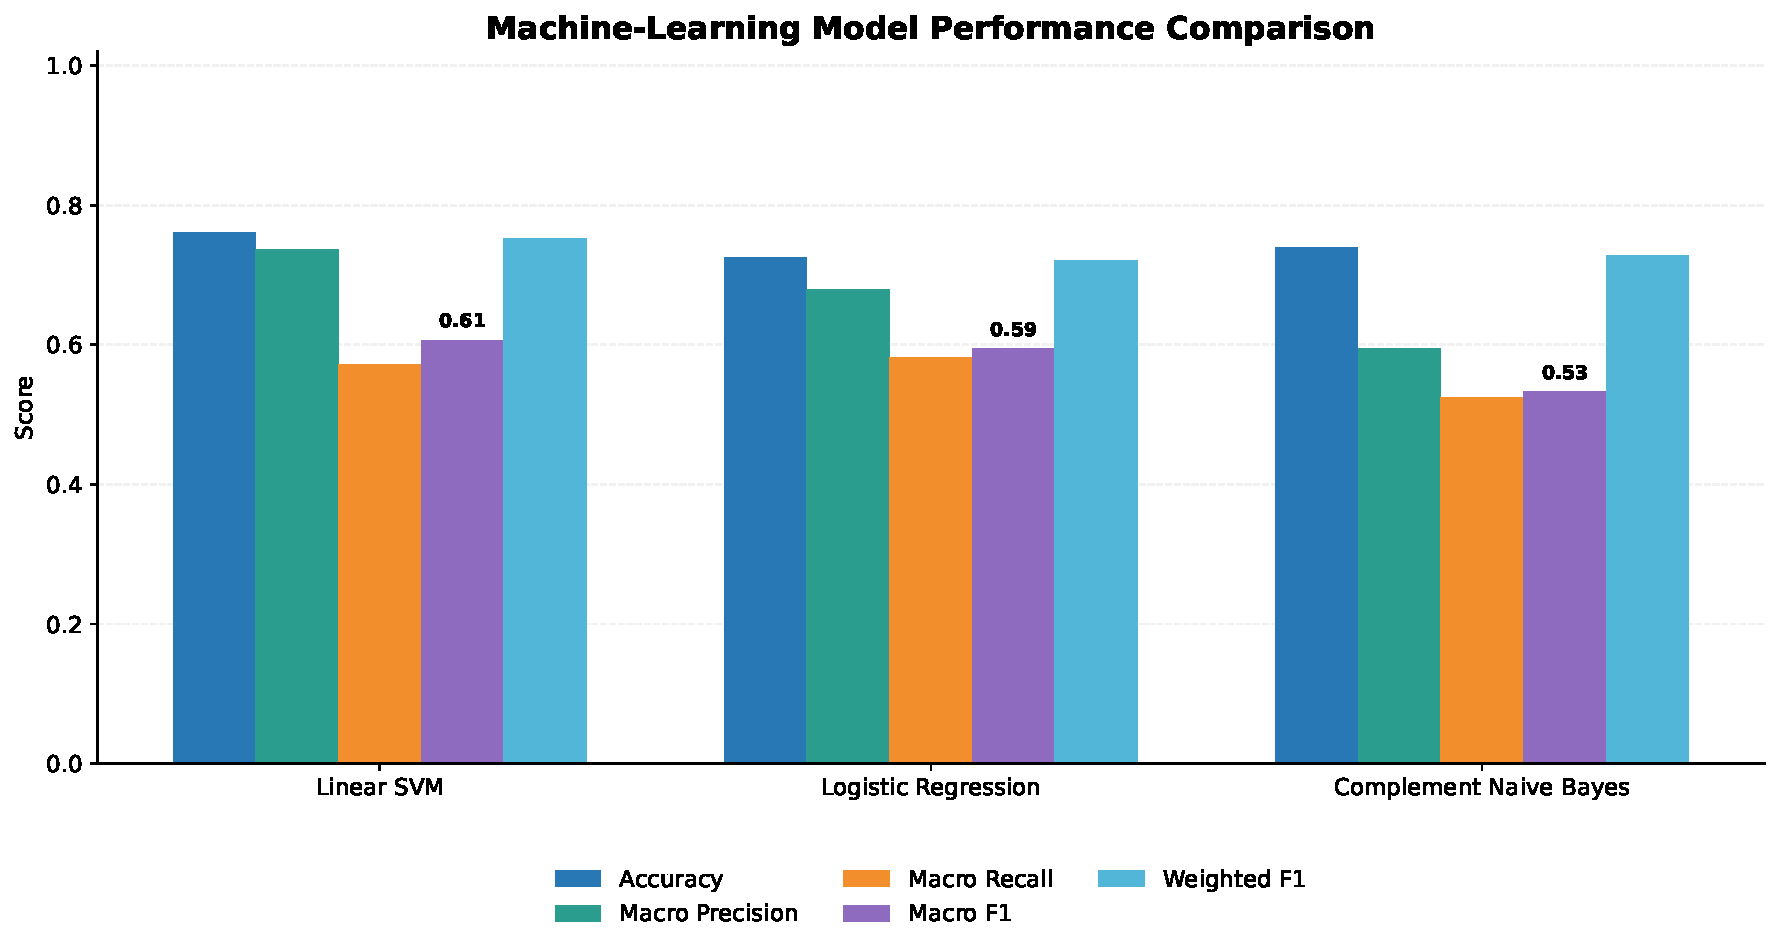
\includegraphics[width=0.78\textwidth]
    {final_model_comparison.pdf}
    \caption{Performance comparison of Linear SVM, Logistic Regression,
    and Complement Naive Bayes on the final incident-classification corpus.}
    \label{fig:model_comparison}
\end{figure*}

\subsection{Class-Wise Performance of Linear SVM}

A single aggregate score does not adequately describe the behavior of the
selected model. Table~\ref{tab:class_report} therefore reports class-level
precision, recall, and F1-score for Linear SVM.

\begin{table*}[!t]
\centering
\caption{Class-Wise Performance of the Selected Linear SVM Model}
\label{tab:class_report}
\renewcommand{\arraystretch}{1.15}
\begin{tabular}{lcccc}
\toprule
\textbf{Incident Category} &
\textbf{Precision} &
\textbf{Recall} &
\textbf{F1-score} &
\textbf{Support} \\
\midrule
Abuse                  & 0.8947 & 0.8095 & 0.8500 & 21 \\
Conflict               & 0.7500 & 0.8276 & 0.7869 & 29 \\
Disease                & 0.8919 & 0.8462 & 0.8684 & 39 \\
Human-Animal Conflict  & 1.0000 & 0.2727 & 0.4286 & 11 \\
Killing                & 0.6364 & 0.6774 & 0.6562 & 31 \\
Other                  & 0.7228 & 0.8111 & 0.7644 & 90 \\
Poisoning              & 1.0000 & 0.3333 & 0.5000 & 3 \\
Rescue                 & 0.0000 & 0.0000 & 0.0000 & 2 \\
\bottomrule
\end{tabular}
\end{table*}

Disease achieved the highest F1-score (0.8684), followed by Abuse (0.8500)
and Conflict (0.7869). The model also performed reasonably well on the
dominant Other category, with an F1-score of 0.7644.

The results become less stable for classes with limited support.
Human-Animal Conflict achieved a precision of 1.0000 but recall of only
0.2727. In other words, predictions assigned to this class were highly
precise within the evaluated data, but many relevant records were not
recovered. Poisoning shows a similar pattern, although its support of only
three records makes the corresponding metrics particularly uncertain.

The Rescue category contained only two observations and obtained zero
precision, recall, and F1-score. This result should not be interpreted as
evidence that Rescue incidents are inherently impossible to classify.
Rather, the available corpus does not contain enough examples for the model
to learn a reliable decision boundary for this category.

Figure~\ref{fig:confusion_matrix} shows the corresponding confusion matrix.

\begin{figure*}[!t]
    \centering
    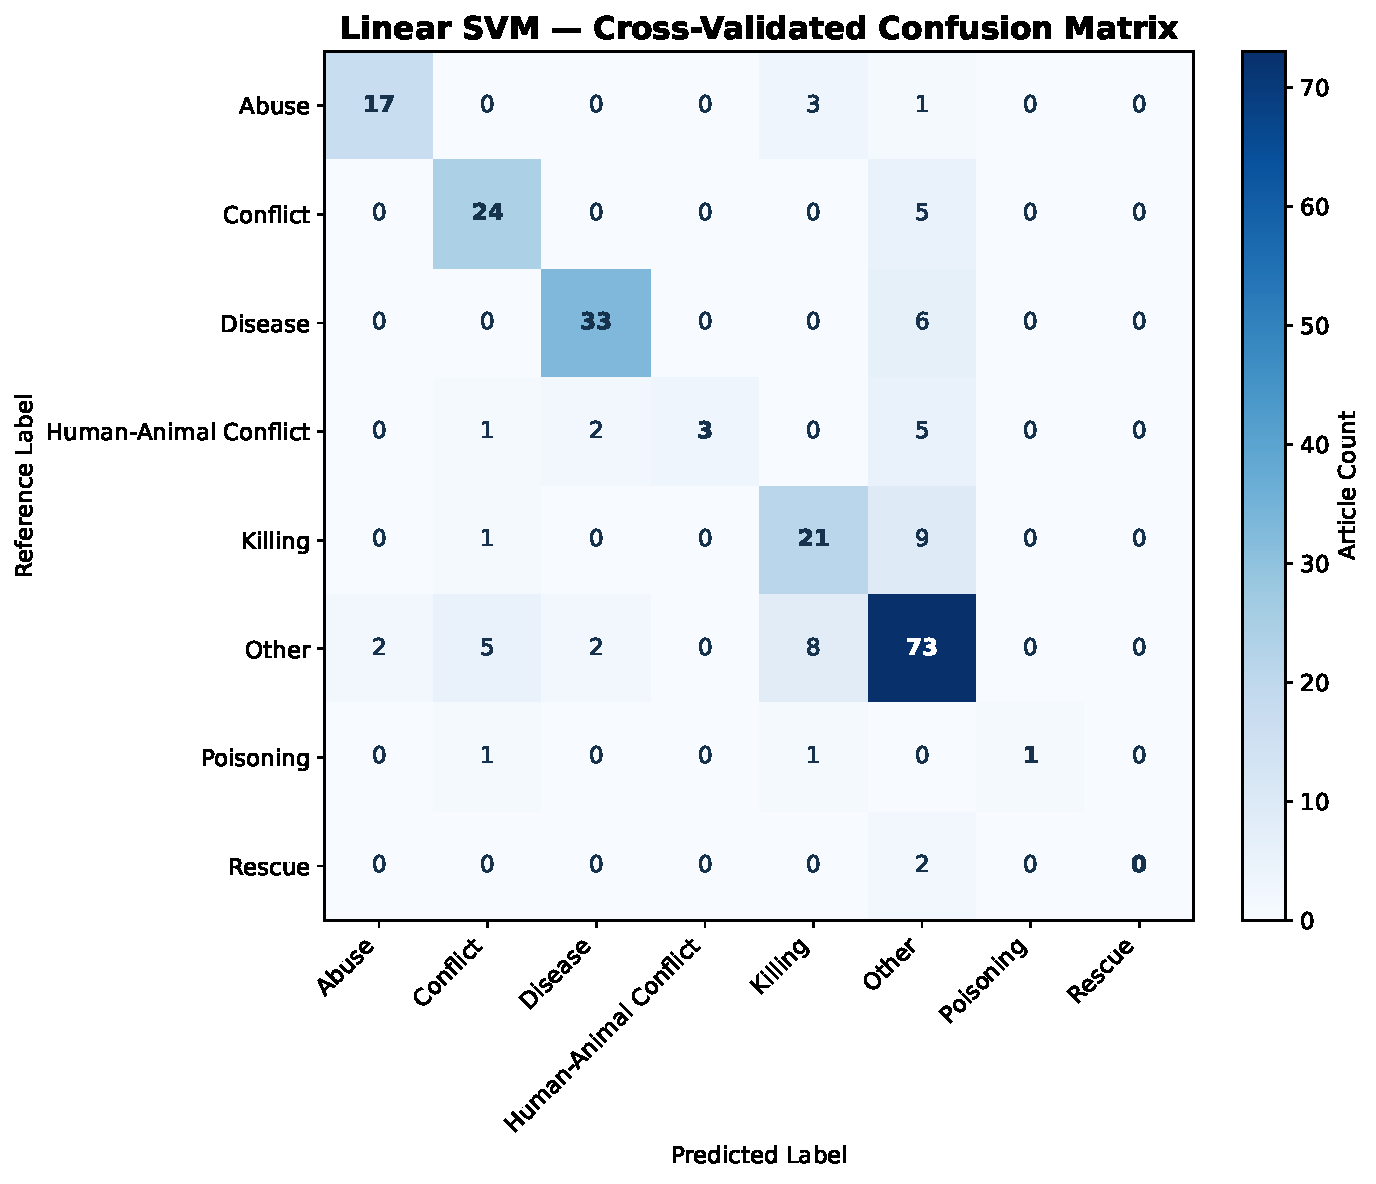
\includegraphics[width=0.72\textwidth]
    {final_confusion_matrix.pdf}
    \caption{Confusion matrix for the selected Linear SVM incident
    classifier.}
    \label{fig:confusion_matrix}
\end{figure*}

\subsection{Interpretation of the Machine-Learning Results}

The results suggest that conventional sparse-text models can recover useful
structure from the refined news corpus, even with a relatively limited
training set. At the same time, the experiment reveals an important data
constraint: performance is closely related to the number and diversity of
examples available for each incident category.

The selected model should therefore be viewed as a proof-of-concept incident
classifier rather than a production-ready automated moderation or welfare
assessment system. Increasing the quantity of carefully reviewed examples,
particularly for Poisoning, Rescue, and Human-Animal Conflict, would be more
valuable than interpreting small differences in model scores as evidence of
complete model reliability.

There is an additional limitation in the evaluation procedure. Most labels in
the corpus originated from rule-based weak supervision, followed by assisted
review of a subset. The cross-validation results therefore measure how well
the models reproduce patterns in this constructed labeling system. They do
not constitute an independent expert-annotated benchmark. This distinction
is retained throughout the interpretation of the results.

\subsection{Incident Distribution in the Final Corpus}

The final 226-record corpus remained dominated by the Other category, with
90 records. Disease accounted for 39 records, Killing for 31, Conflict for
29, and Abuse for 21. Human-Animal Conflict was represented by 11 records,
while Poisoning and Rescue contained only three and two records,
respectively.

Figure~\ref{fig:incident_distribution} illustrates this distribution.

\begin{figure}[!t]
    \centering
    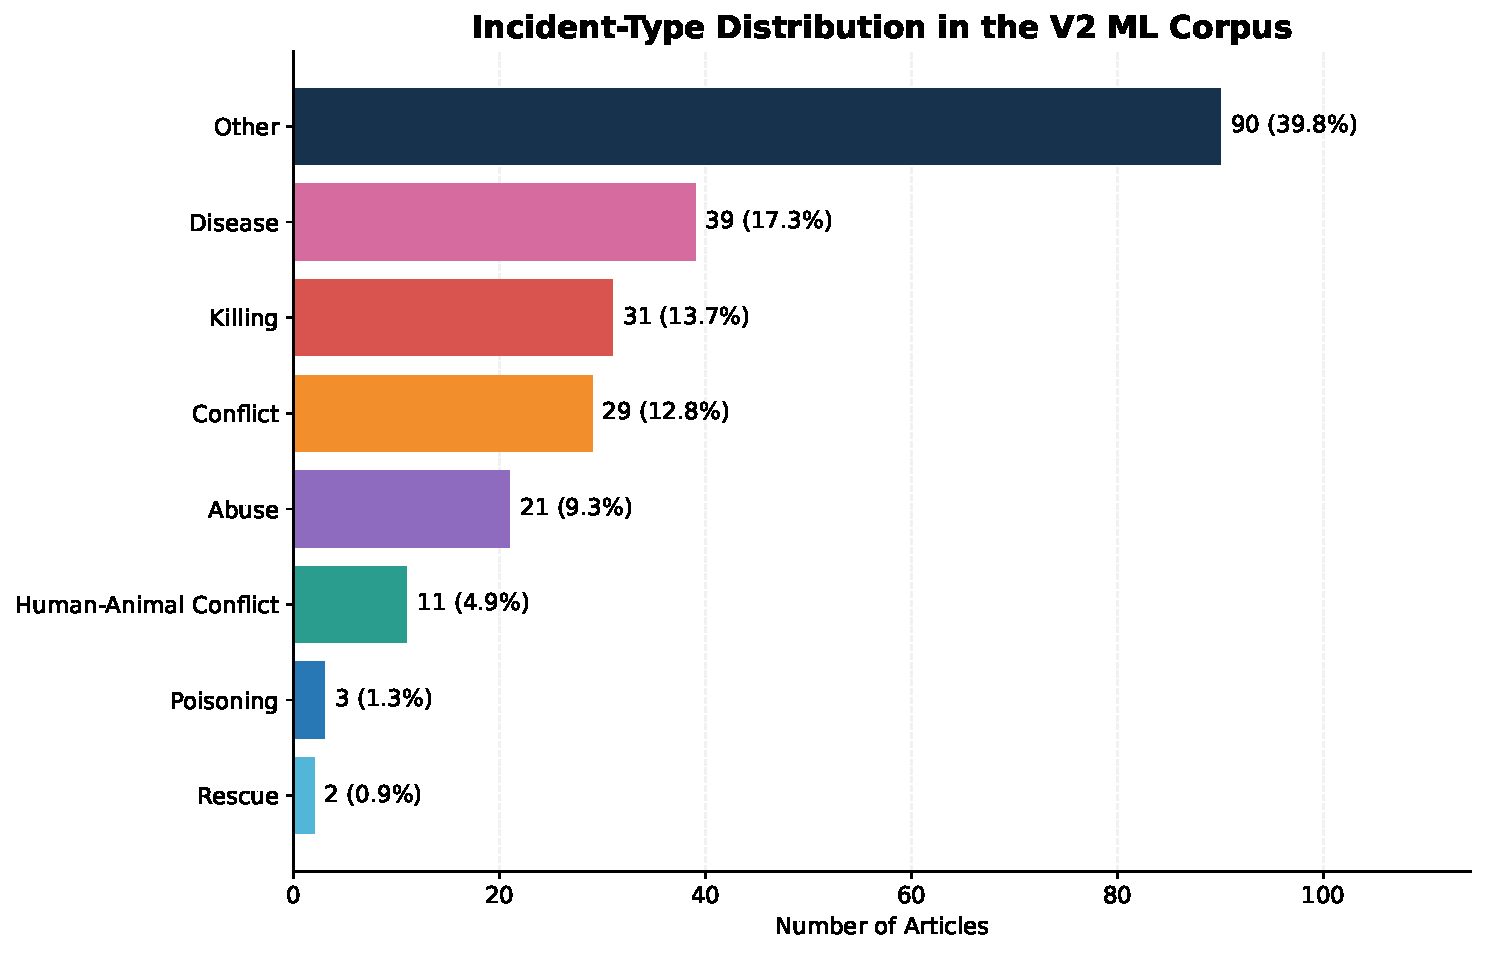
\includegraphics[width=\columnwidth]
    {final_incident_distribution.pdf}
    \caption{Distribution of incident categories in the final
    226-record machine-learning corpus.}
    \label{fig:incident_distribution}
\end{figure}

This distribution provides useful context for interpreting the model
performance. It also illustrates a practical challenge in media-derived
datasets: some incident types are reported or captured far more frequently
than others. The observed counts should therefore be interpreted as the
composition of the collected news corpus, not as the true prevalence of
stray-animal incidents across Bangladesh.

\subsection{Temporal Distribution}

The Bangladesh-primary news collection spans multiple years, with the final
analytical corpus reflecting records available through the implemented
collection process. Figure~\ref{fig:yearly_trend} presents the temporal
distribution of the retained incidents.

\begin{figure*}[!t]
    \centering
    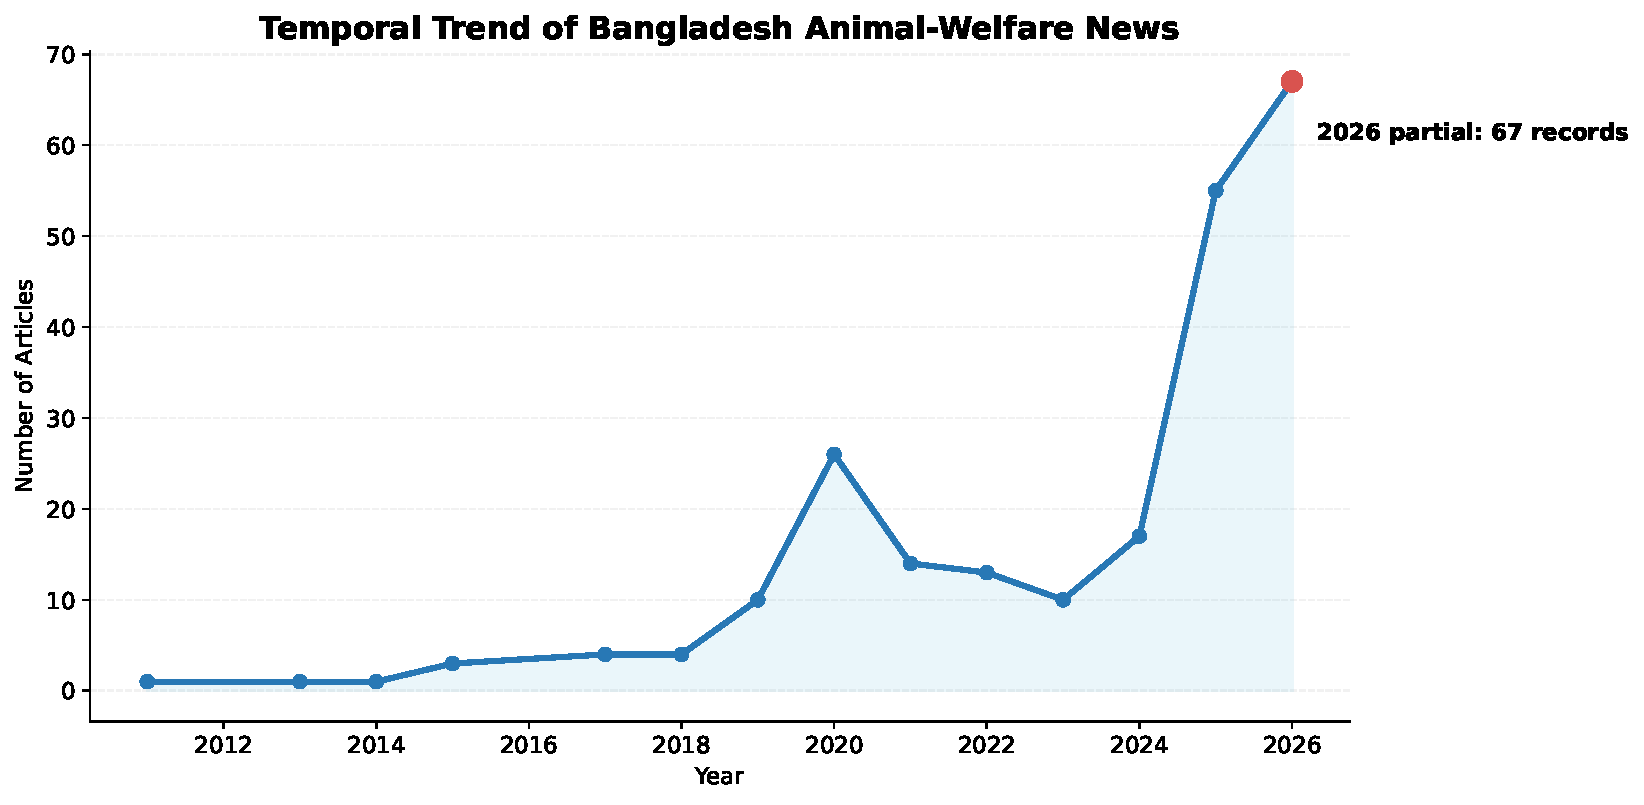
\includegraphics[width=0.80\textwidth]
    {final_yearly_trend.pdf}
    \caption{Temporal distribution of incident records in the refined
    Bangladesh-focused news corpus.}
    \label{fig:yearly_trend}
\end{figure*}

The temporal pattern should be interpreted cautiously. The collection was
constructed through retrospective news retrieval rather than a fixed,
prospective surveillance system. Changes in news availability, search-engine
indexing, source coverage, and reporting practices may therefore influence
the number of records observed in different years.

In addition, records from 2026 represent only the period captured during data
collection and should not be compared with completed calendar years as if
they represented equivalent observation windows. For these reasons, the
temporal visualization is used descriptively rather than as evidence of a
causal increase or decrease in the underlying national incidence rate.

\subsection{SARI V2 Risk Distribution}

SARI V2 was calculated independently from the supervised model target. Across
the 226 records, the mean score was 1.550 with a standard deviation of 1.344.
The median was 2.100, and scores ranged from 0.100 to 5.500.

Using the predefined descriptive thresholds, 191 records were categorized as
Low risk and 35 as Medium risk. No record reached the High-risk threshold of
6.0.

\begin{table}[!t]
\centering
\caption{Summary of SARI V2 Scores}
\label{tab:sari_summary}
\renewcommand{\arraystretch}{1.15}
\begin{tabular}{lr}
\toprule
\textbf{Measure} & \textbf{Value} \\
\midrule
Number of records & 226 \\
Mean score         & 1.550 \\
Standard deviation & 1.344 \\
Median             & 2.100 \\
Minimum            & 0.100 \\
Maximum            & 5.500 \\
\midrule
Low risk           & 191 \\
Medium risk        & 35 \\
High risk          & 0 \\
\bottomrule
\end{tabular}
\end{table}

\begin{figure}[!t]
    \centering
    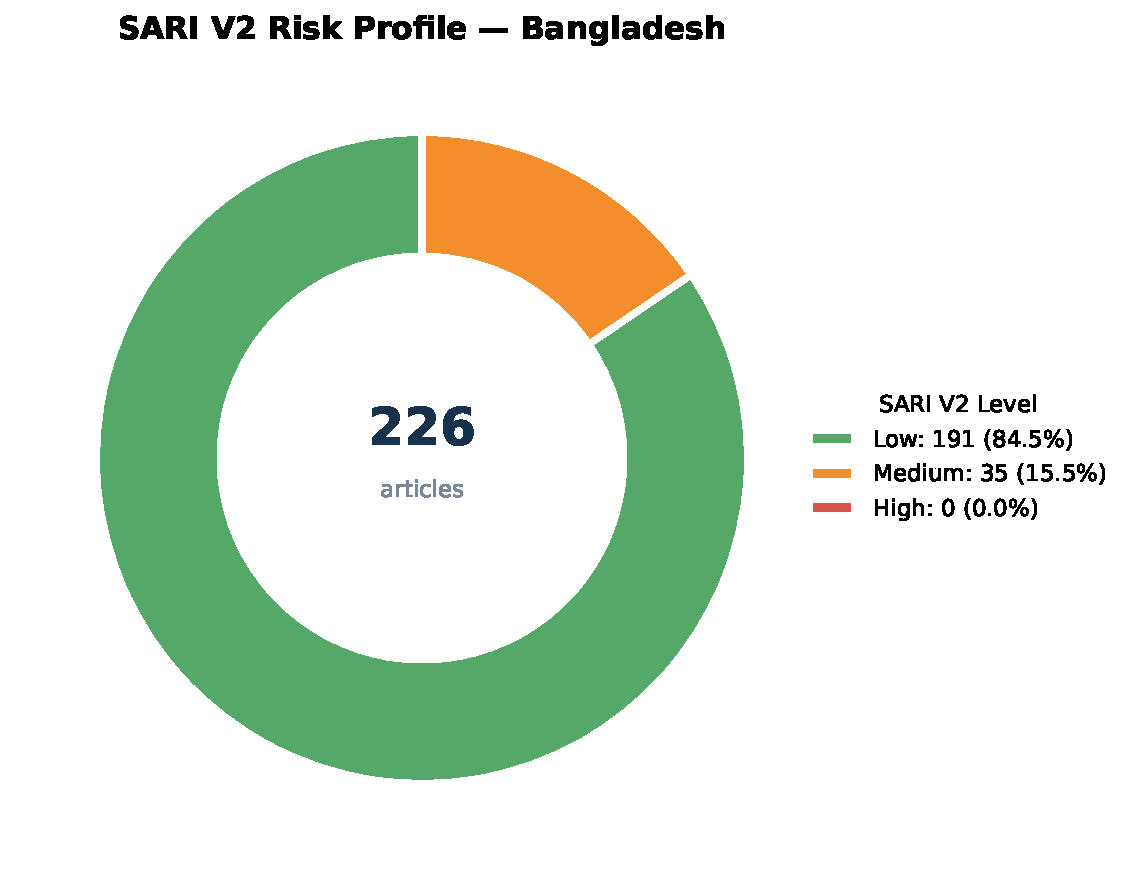
\includegraphics[width=\columnwidth]
    {final_sari_risk_donut.pdf}
    \caption{Distribution of descriptive SARI V2 risk levels across the
    final news corpus.}
    \label{fig:sari_distribution}
\end{figure}

The absence of High-risk records is an actual outcome of the implemented
scoring procedure and was retained without adjusting the thresholds to force
a more visually balanced distribution. The highest observed score was 5.500,
which remained below the predefined High-risk boundary.

This finding also highlights the need to treat SARI V2 as an interpretable
heuristic rather than a calibrated probability model. Its present value lies
in ranking and summarizing textual risk indicators consistently; the weights
and thresholds require external validation before the score could support
high-stakes operational decisions.

\subsection{SARI V2 by Incident Category}

Average SARI V2 scores differed considerably across incident categories.
Poisoning had the highest mean score at 4.833, followed by Human-Animal
Conflict at 3.436. Abuse averaged 2.971, Killing 2.645, Disease 2.305, and
Conflict 1.503. Other and Rescue produced substantially lower mean values of
0.222 and 0.100, respectively.

\begin{table}[!t]
\centering
\caption{Mean SARI V2 Score by Incident Category}
\label{tab:sari_incident}
\renewcommand{\arraystretch}{1.12}
\begin{tabular}{lr}
\toprule
\textbf{Incident Category} & \textbf{Mean SARI V2} \\
\midrule
Poisoning               & 4.833 \\
Human-Animal Conflict   & 3.436 \\
Abuse                   & 2.971 \\
Killing                 & 2.645 \\
Disease                 & 2.305 \\
Conflict                & 1.503 \\
Other                   & 0.222 \\
Rescue                  & 0.100 \\
\bottomrule
\end{tabular}
\end{table}

\begin{figure}[!t]
    \centering
    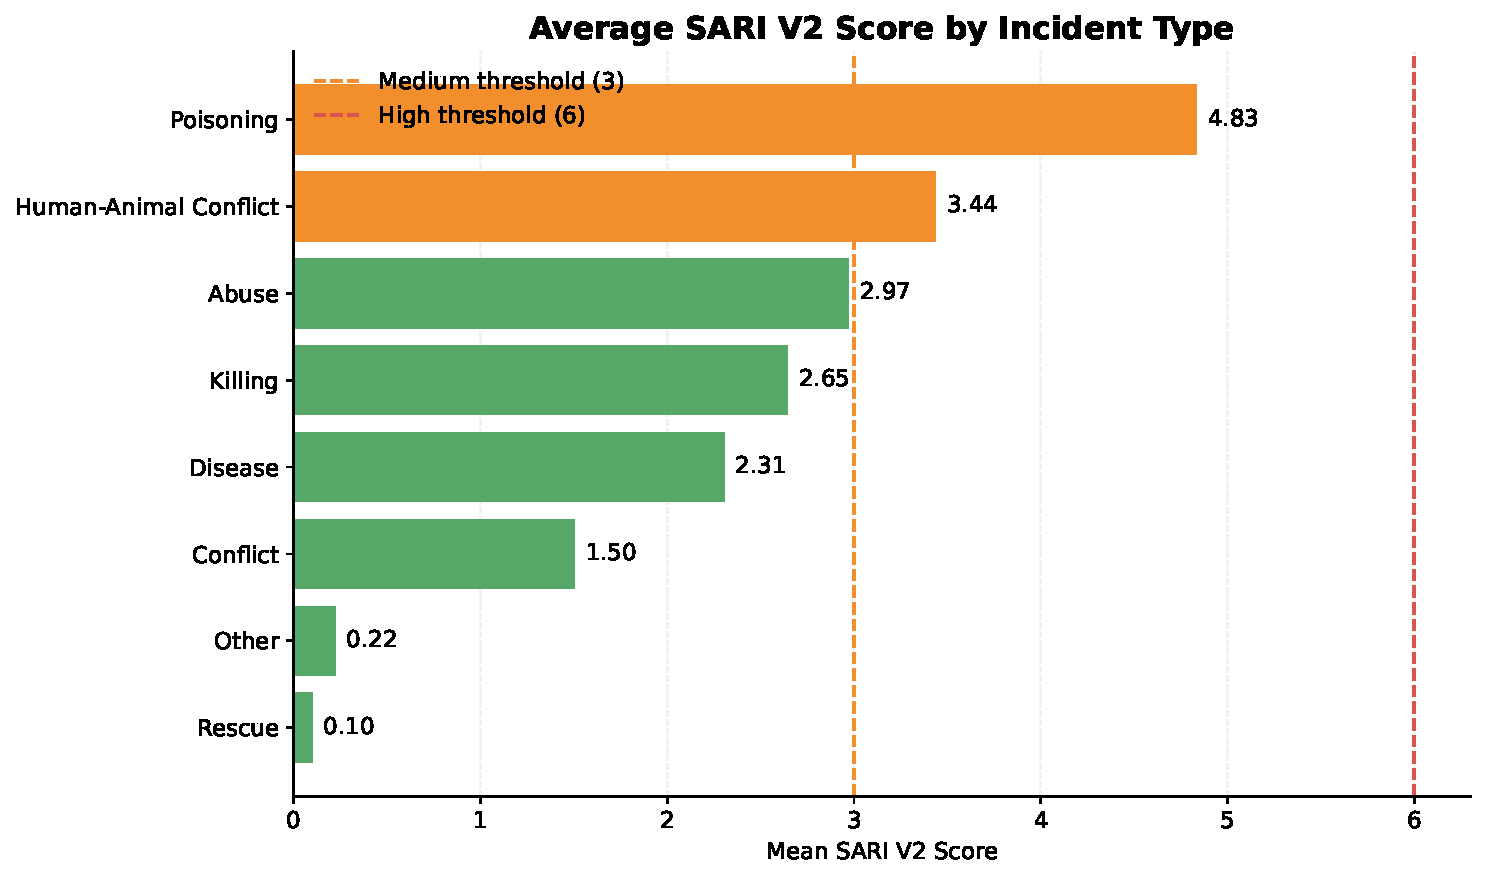
\includegraphics[width=\columnwidth]
    {final_mean_sari_by_incident.pdf}
    \caption{Mean SARI V2 score across incident categories.}
    \label{fig:sari_incident}
\end{figure}

These differences are partly expected because incident context contributes
directly to the SARI V2 heuristic. They should therefore not be interpreted
as an independently discovered causal relationship between incident class
and welfare risk. Instead, the comparison demonstrates how the implemented
risk logic prioritizes different combinations of textual and contextual
signals.

\FloatBarrier

% =========================================================
% VIII. FIELD SURVEY RESULTS
% =========================================================

\section{Field Survey Results}

The field-survey component provides a localized view of stray-animal welfare
conditions in Badda, Dhaka. A total of 325 animals were observed across Uttar
Badda, Dokkhin Badda, Moddho Badda, and Jheelpar. Because the survey was not
designed as a probability sample of Bangladesh, all percentages reported in
this section refer only to the surveyed animals.

\subsection{Animal Composition and Spatial Coverage}

Dogs represented the overwhelming majority of observations, with 322 dogs
and 3 cats. Uttar Badda accounted for 219 observations, followed by Dokkhin
Badda with 43, Moddho Badda with 39, and Jheelpar with 24.

The strong concentration of observations in Uttar Badda indicates that the
field sample is spatially uneven. This is important when interpreting
location-specific rates, since local percentages can be influenced by the
number of surveyed animals available in each area.

\begin{table}[!t]
\centering
\caption{Survey Distribution by Location}
\label{tab:survey_locations}
\renewcommand{\arraystretch}{1.15}
\begin{tabular}{lr}
\toprule
\textbf{Location} & \textbf{Observed Animals} \\
\midrule
Uttar Badda   & 219 \\
Dokkhin Badda & 43 \\
Moddho Badda  & 39 \\
Jheelpar       & 24 \\
\midrule
\textbf{Total} & \textbf{325} \\
\bottomrule
\end{tabular}
\end{table}

\subsection{Observed Health Condition}

The survey recorded three broad health-condition categories. Among the 325
animals, 232 were recorded as Healthy, 65 as Underweight / Malnourished, and
28 as Starved.

Combining the latter two categories gives 93 animals with an observed
nutritional health concern. This corresponds to

\begin{equation}
\frac{65+28}{325}\times100 = 28.62\%.
\end{equation}

Therefore, approximately 28.62\% of the surveyed animals showed an observed
nutritional health concern according to the field-survey categories.

This measure should be interpreted cautiously. It reflects visual or
field-level observations and is not equivalent to a veterinary diagnosis or
an estimate of disease prevalence.

\begin{figure}[!t]
    \centering
    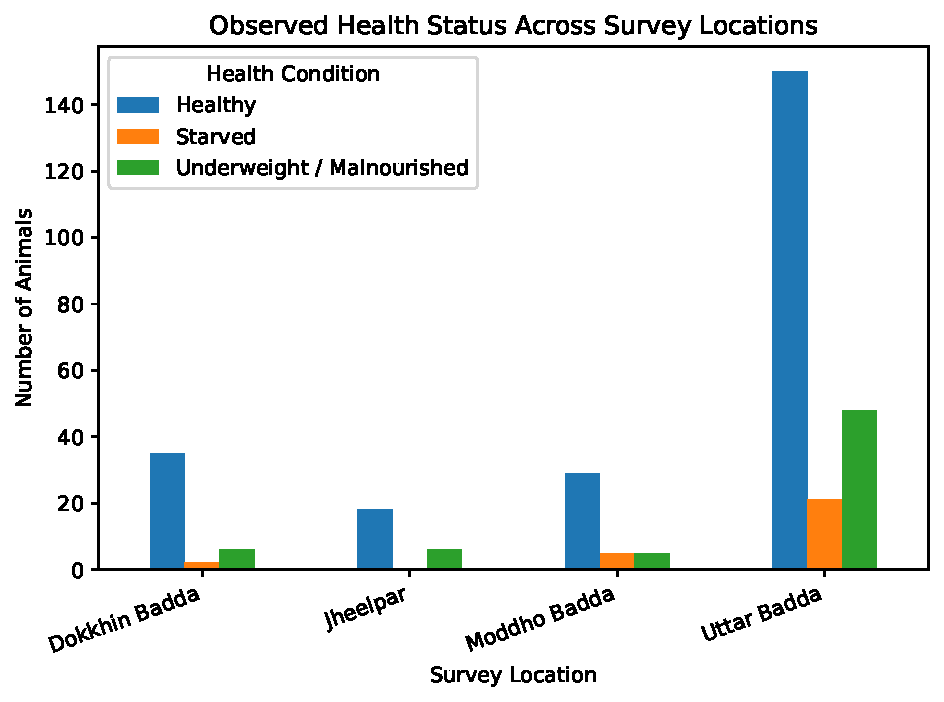
\includegraphics[width=\columnwidth]
    {final_survey_health_status_by_location.pdf}
    \caption{Observed health-status distribution across the surveyed
    Badda locations.}
    \label{fig:survey_health_status}
\end{figure}

\subsection{Vaccination Coverage}

Only 32 of the 325 surveyed animals were recorded as vaccinated, while 293
were recorded as not vaccinated. The observed vaccination rate was therefore

\begin{equation}
Vaccination\ Rate =
\frac{32}{325}\times100
=
9.85\%.
\end{equation}

The result indicates low vaccination coverage within the surveyed sample.
Given the relevance of dog vaccination to rabies prevention, this represents
a notable intervention gap within the pilot area. However, the result should
not be generalized beyond the observed sample.

Location-wise analysis showed that no vaccinated animals were recorded among
the surveyed animals in Dokkhin Badda. This statement refers specifically to
the collected sample and does not imply that vaccination coverage is
literally zero across the entire Dokkhin Badda area.

\subsection{Sterilization Coverage}

Sterilization coverage was similarly limited. Among the 325 animals, 34 were
recorded as sterilized and 291 as not sterilized, corresponding to an observed
sterilization rate of

\begin{equation}
Sterilization\ Rate =
\frac{34}{325}\times100
=
10.46\%.
\end{equation}

Location-level analysis found no sterilized animals among the surveyed
Jheelpar observations. As with vaccination, this finding is descriptive of
the sampled animals and should not be interpreted as an area-wide prevalence
estimate.

Figure~\ref{fig:survey_intervention} compares vaccination and sterilization
coverage across the surveyed locations.

\begin{figure*}[!t]
    \centering
    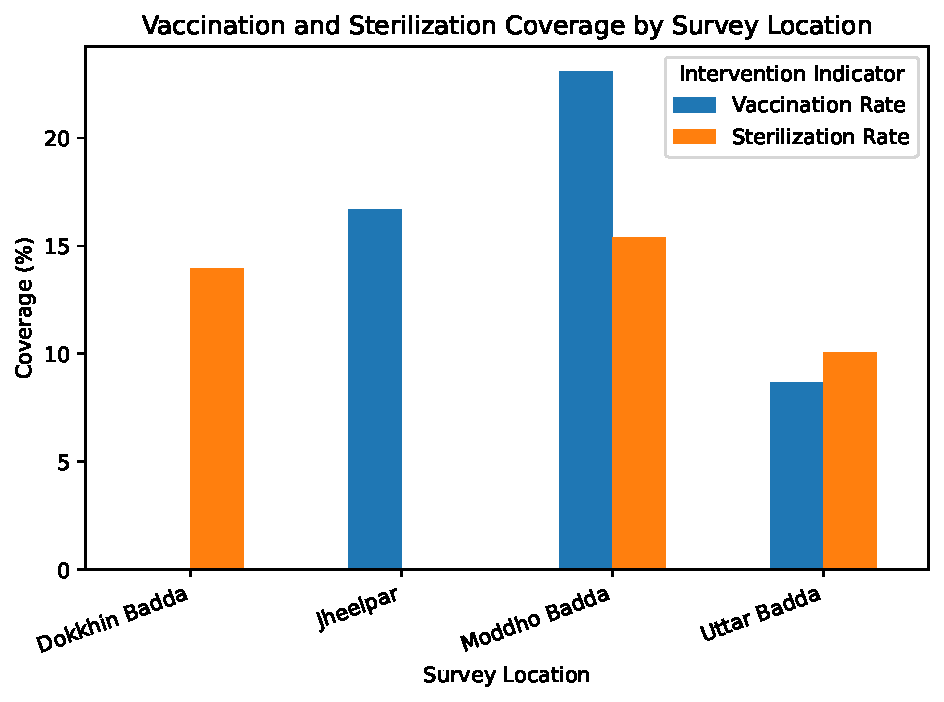
\includegraphics[width=0.68\textwidth]
    {final_survey_intervention_coverage_by_location.pdf}
    \caption{Observed vaccination and sterilization coverage across the four
    Badda pilot locations.}
    \label{fig:survey_intervention}
\end{figure*}

\subsection{Location-Specific Welfare Concerns}

The highest observed nutritional health-concern rate was found in Uttar Badda,
where 31.51\% of the surveyed animals were categorized as either
Underweight / Malnourished or Starved.

Figure~\ref{fig:health_concern_location} illustrates the location-level
distribution of this indicator.

\begin{figure}[!t]
    \centering
    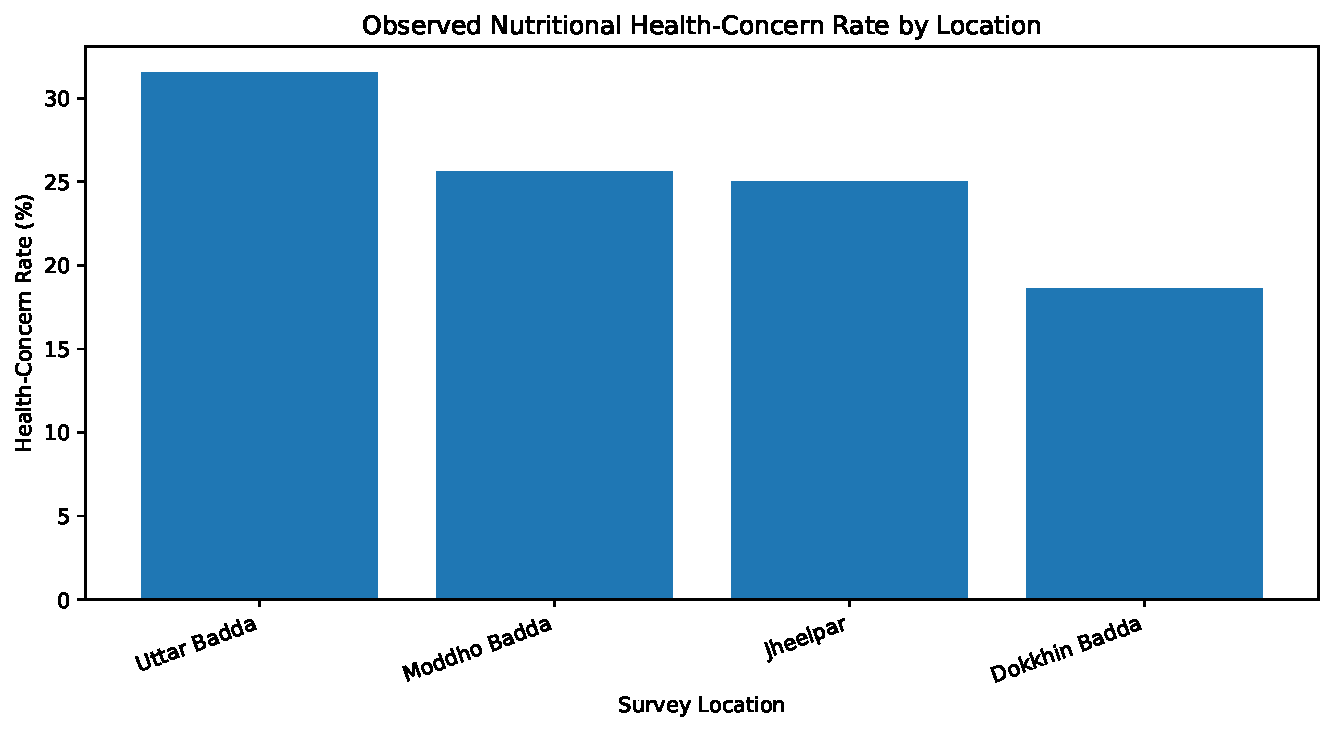
\includegraphics[width=\columnwidth]
    {final_survey_health_concern_by_location.pdf}
    \caption{Observed nutritional health-concern rate by survey location.}
    \label{fig:health_concern_location}
\end{figure}

The location-specific results should be interpreted jointly with the sample
sizes. Uttar Badda has the largest number of observations and therefore
dominates the overall survey composition. Smaller areas such as Jheelpar have
fewer observations, which makes their percentages more sensitive to small
changes in the underlying counts.

\subsection{Human-Directed Behavior}

Most surveyed animals were recorded as Friendly toward humans. A total of 259
animals were categorized as Friendly, 50 as Scared, and 8 as Aggressive.
A small number of records included combined behavioral descriptions.

This pattern suggests that overt aggression was relatively uncommon in the
surveyed sample. Nevertheless, behavior recorded during a field observation
can be influenced by the immediate environment, presence of people, food,
injury, fear, or other situational factors. The survey therefore treats
behavior as a descriptive field observation rather than a stable behavioral
diagnosis.

\subsection{Visible Health Issues}

The raw survey included free-text descriptions of visible health problems.
These descriptions varied substantially in wording and detail. During
preprocessing, similar descriptions were grouped into broader categories such
as skin-related issues, injury, mobility concerns, eye or ear problems, and
other visible conditions.

The normalization process was used to support descriptive analysis while
avoiding the assumption that surveyor observations constitute confirmed
clinical diagnoses.

\subsection{Field-Level Intervention Gap}

The combination of low observed vaccination and sterilization coverage,
together with the presence of animals showing nutritional health concerns,
suggests that the pilot area contains identifiable intervention gaps.

Figure~\ref{fig:intervention_gap} summarizes these field-level indicators.

\begin{figure}[!t]
    \centering
    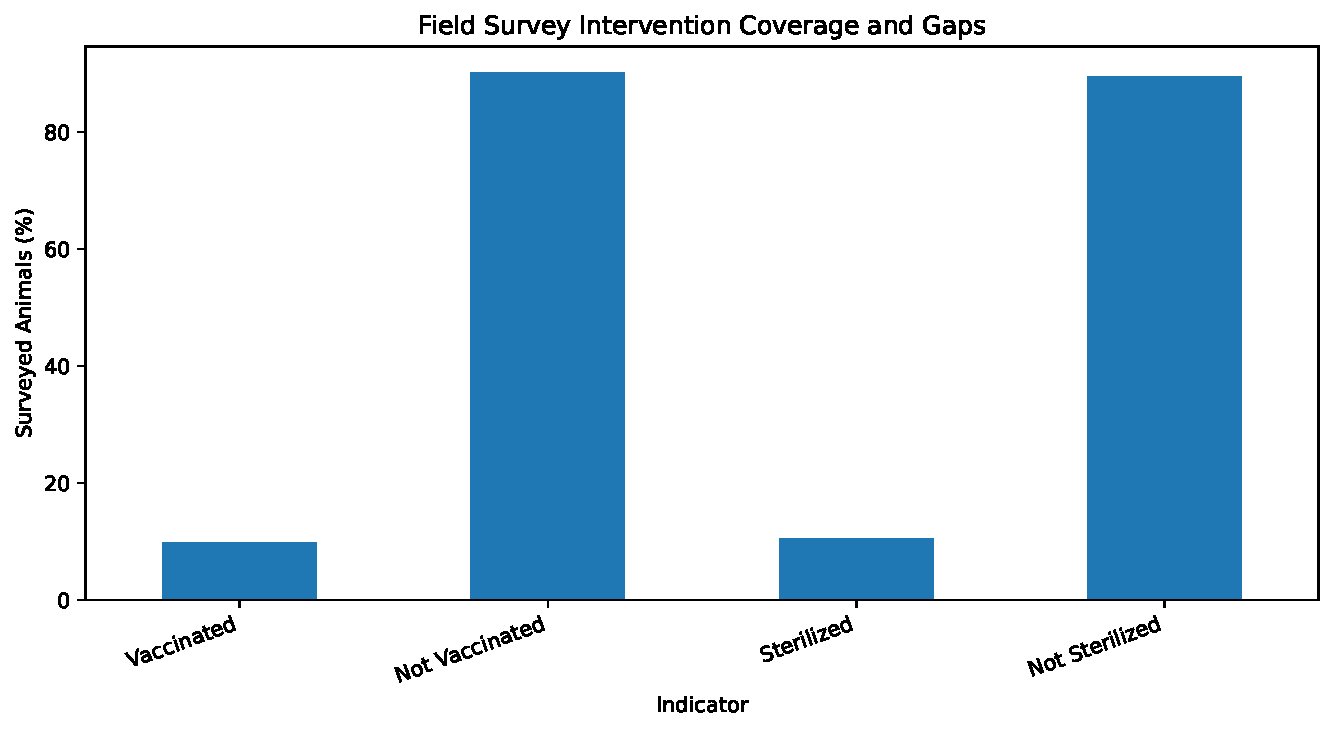
\includegraphics[width=\columnwidth]
    {final_survey_intervention_gap.pdf}
    \caption{Summary of observed intervention gaps in the Badda pilot
    field-survey sample.}
    \label{fig:intervention_gap}
\end{figure}

The purpose of this analysis is not to rank neighborhoods as ``good'' or
``bad.'' Instead, the indicators illustrate how a local animal-welfare
initiative could use structured field observations to prioritize follow-up
surveying, vaccination campaigns, sterilization support, feeding assistance,
or veterinary outreach.

% =========================================================
% IX. INTEGRATED WELFARE INTELLIGENCE
% =========================================================

\section{Integrated Welfare Intelligence}

The central contribution of the proposed framework is the combination of two
different but complementary forms of evidence. The news component captures
reported incidents over a broader Bangladesh-focused information space,
whereas the field component captures direct observations from a localized
Badda pilot area.

These sources are not directly interchangeable. News reports are shaped by
editorial selection, search visibility, public attention, and the severity or
newsworthiness of events. Field surveys, in contrast, provide direct
observations but are geographically limited and depend on the coverage of the
survey team.

For this reason, the framework does not attempt to combine the two datasets
into a single row-level model. Instead, their outputs are interpreted jointly
to support welfare-oriented decision making.

\subsection{News Intelligence Contribution}

The news branch contributes three principal outputs:

\begin{itemize}
    \item predicted incident categories from the selected Linear SVM model;
    \item descriptive incident and temporal patterns from the refined corpus;
    \item SARI V2 scores that provide an interpretable heuristic measure of
    textual and contextual severity.
\end{itemize}

Together, these outputs help organize a large set of unstructured news records
into a more structured representation of reported animal-welfare events.

\subsection{Field Intelligence Contribution}

The field branch contributes direct observations related to animal condition
and intervention coverage. In the Badda pilot sample, vaccination coverage
was 9.85\%, sterilization coverage was 10.46\%, and 28.62\% of animals were
recorded as underweight/malnourished or starved.

These indicators address questions that the news corpus cannot answer
reliably. News reports may describe severe or unusual events, but they do not
provide systematic information on the routine vaccination, sterilization, or
nutritional condition of free-roaming animals.

\subsection{Complementary Interpretation}

The two evidence streams therefore operate at different analytical levels.
The news branch is event-oriented, while the field branch is
condition-oriented.

This distinction can be summarized as

\begin{equation}
News\ Intelligence \rightarrow Reported\ Events,
\end{equation}

\begin{equation}
Field\ Intelligence \rightarrow Observed\ Conditions.
\end{equation}

The combined framework uses both perspectives to support a broader welfare
assessment.

For example, a welfare organization may use incident intelligence to identify
recurring categories of concern while using field observations to determine
where vaccination, sterilization, nutritional support, or veterinary
assessment may be most urgently needed.

\subsection{Dual-Source Evidence Overview}

Figure~\ref{fig:v2_architecture} presents a consolidated visual summary of the two
evidence streams.

\begin{figure*}[!t]
    \centering
    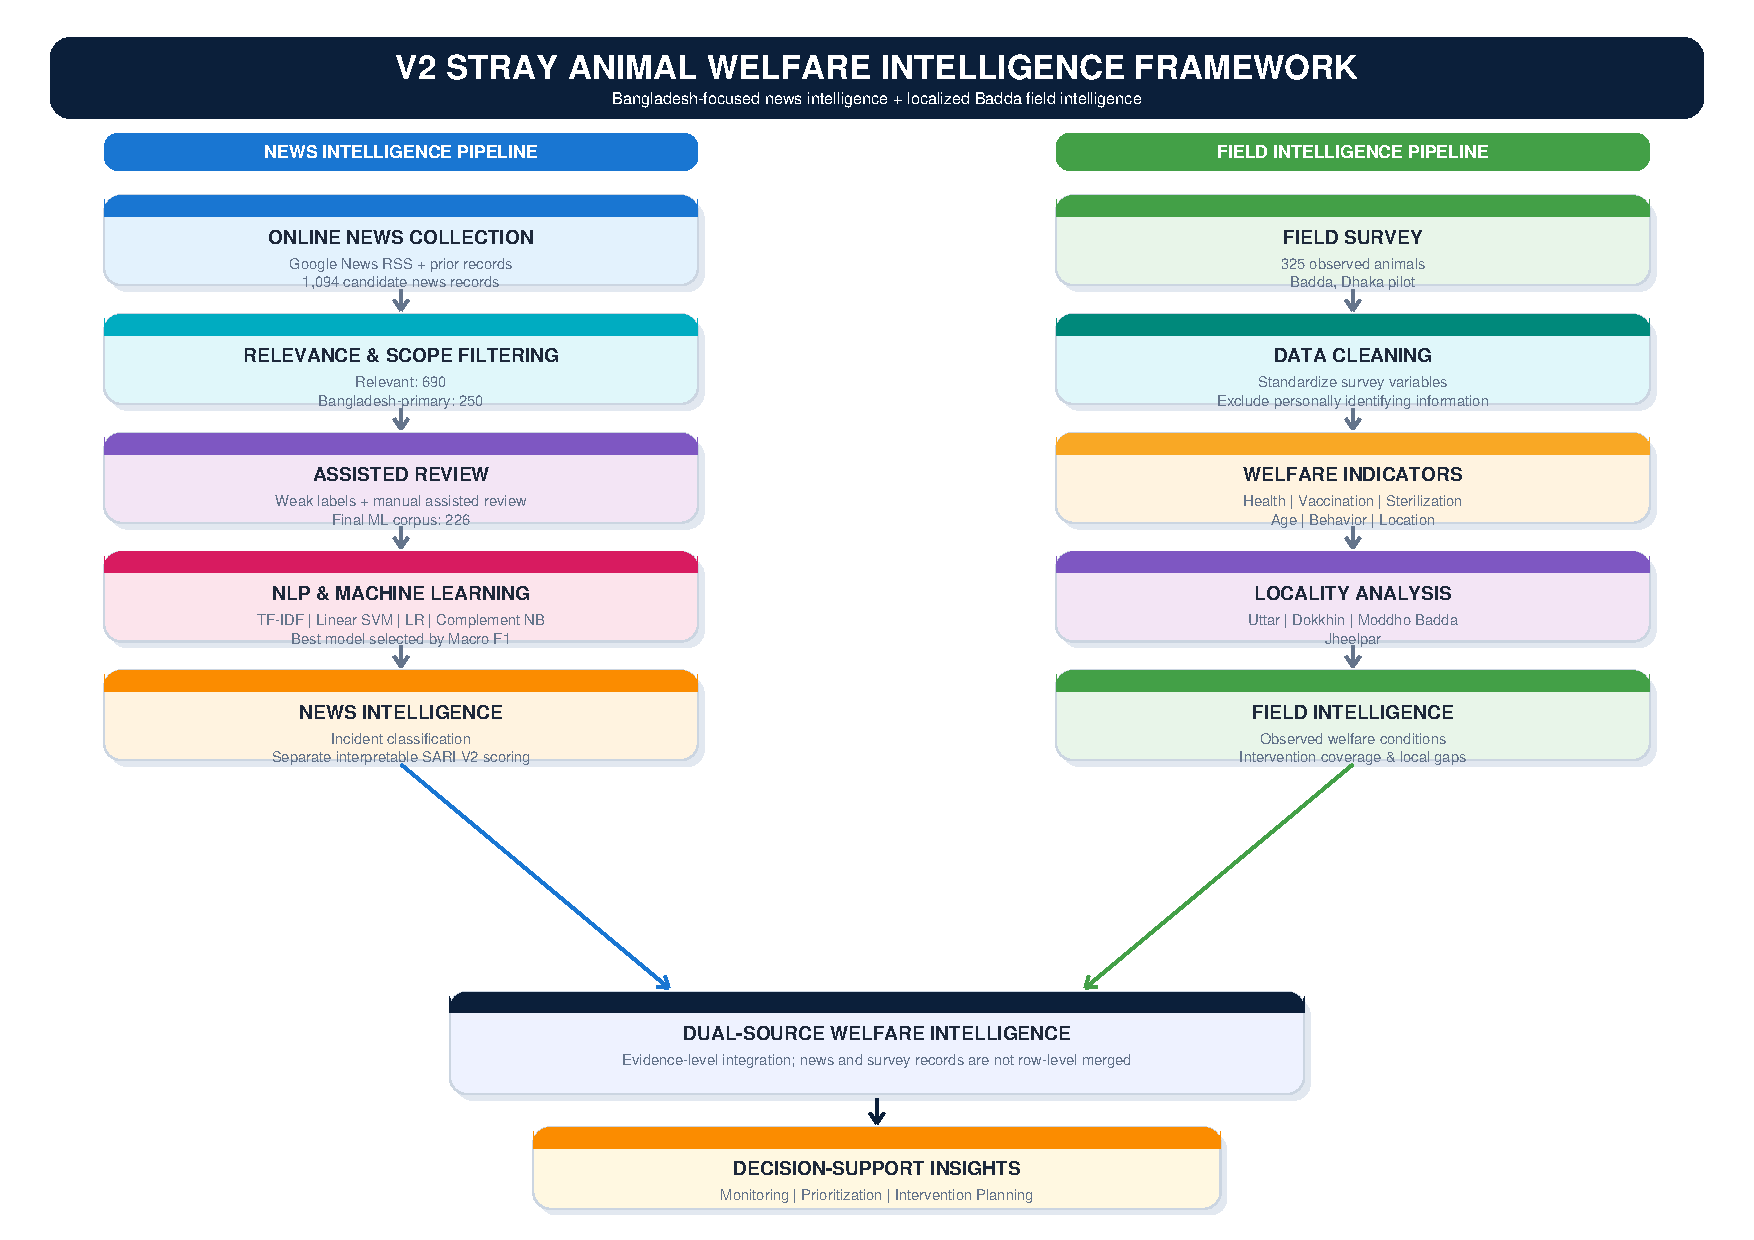
\includegraphics[width=0.95\textwidth]
    {v2_welfare_intelligence_architecture_colorful.pdf}
    \caption{Architecture of the proposed V2 stray animal welfare intelligence framework. 
    The news branch performs relevance filtering, Bangladesh-specific scope refinement, 
    assisted review, TF-IDF-based incident classification, and separate SARI V2 scoring. 
    The field branch analyzes observed welfare indicators from the Badda pilot survey. 
    Both branches are integrated at the evidence level to support monitoring, prioritization, 
    and intervention planning.}
    \label{fig:v2_architecture}
\end{figure*}

The integrated view should be interpreted as a decision-support framework,
not as a national epidemiological surveillance system. The news corpus is not
a census of all incidents in Bangladesh, and the field survey is not
nationally representative. The framework instead demonstrates how two
different forms of imperfect but useful evidence can be organized into a
single analytical workflow.

\FloatBarrier
% =========================================================
% X. MODEL INTERPRETABILITY
% =========================================================

\section{Model Interpretability}

Predictive performance alone provides limited value in a welfare-intelligence
system if the basis of a model's decisions cannot be inspected. For this
reason, the selected Linear SVM was examined through its learned feature
weights. Since the classifier operates on TF--IDF representations, terms with
larger positive coefficients for a particular class provide an indication of
which textual features most strongly influence that class within the fitted
model.

The analysis was performed on the trained Linear SVM stored after model
selection. For each incident category, the highest-weighted TF--IDF features
were extracted and ranked. This provides a lightweight and model-specific
form of interpretability without introducing a separate explanation model.

Figure~\ref{fig:top_features} presents the most influential textual features
identified for the incident classes.

\begin{figure*}[!t]
    \centering
    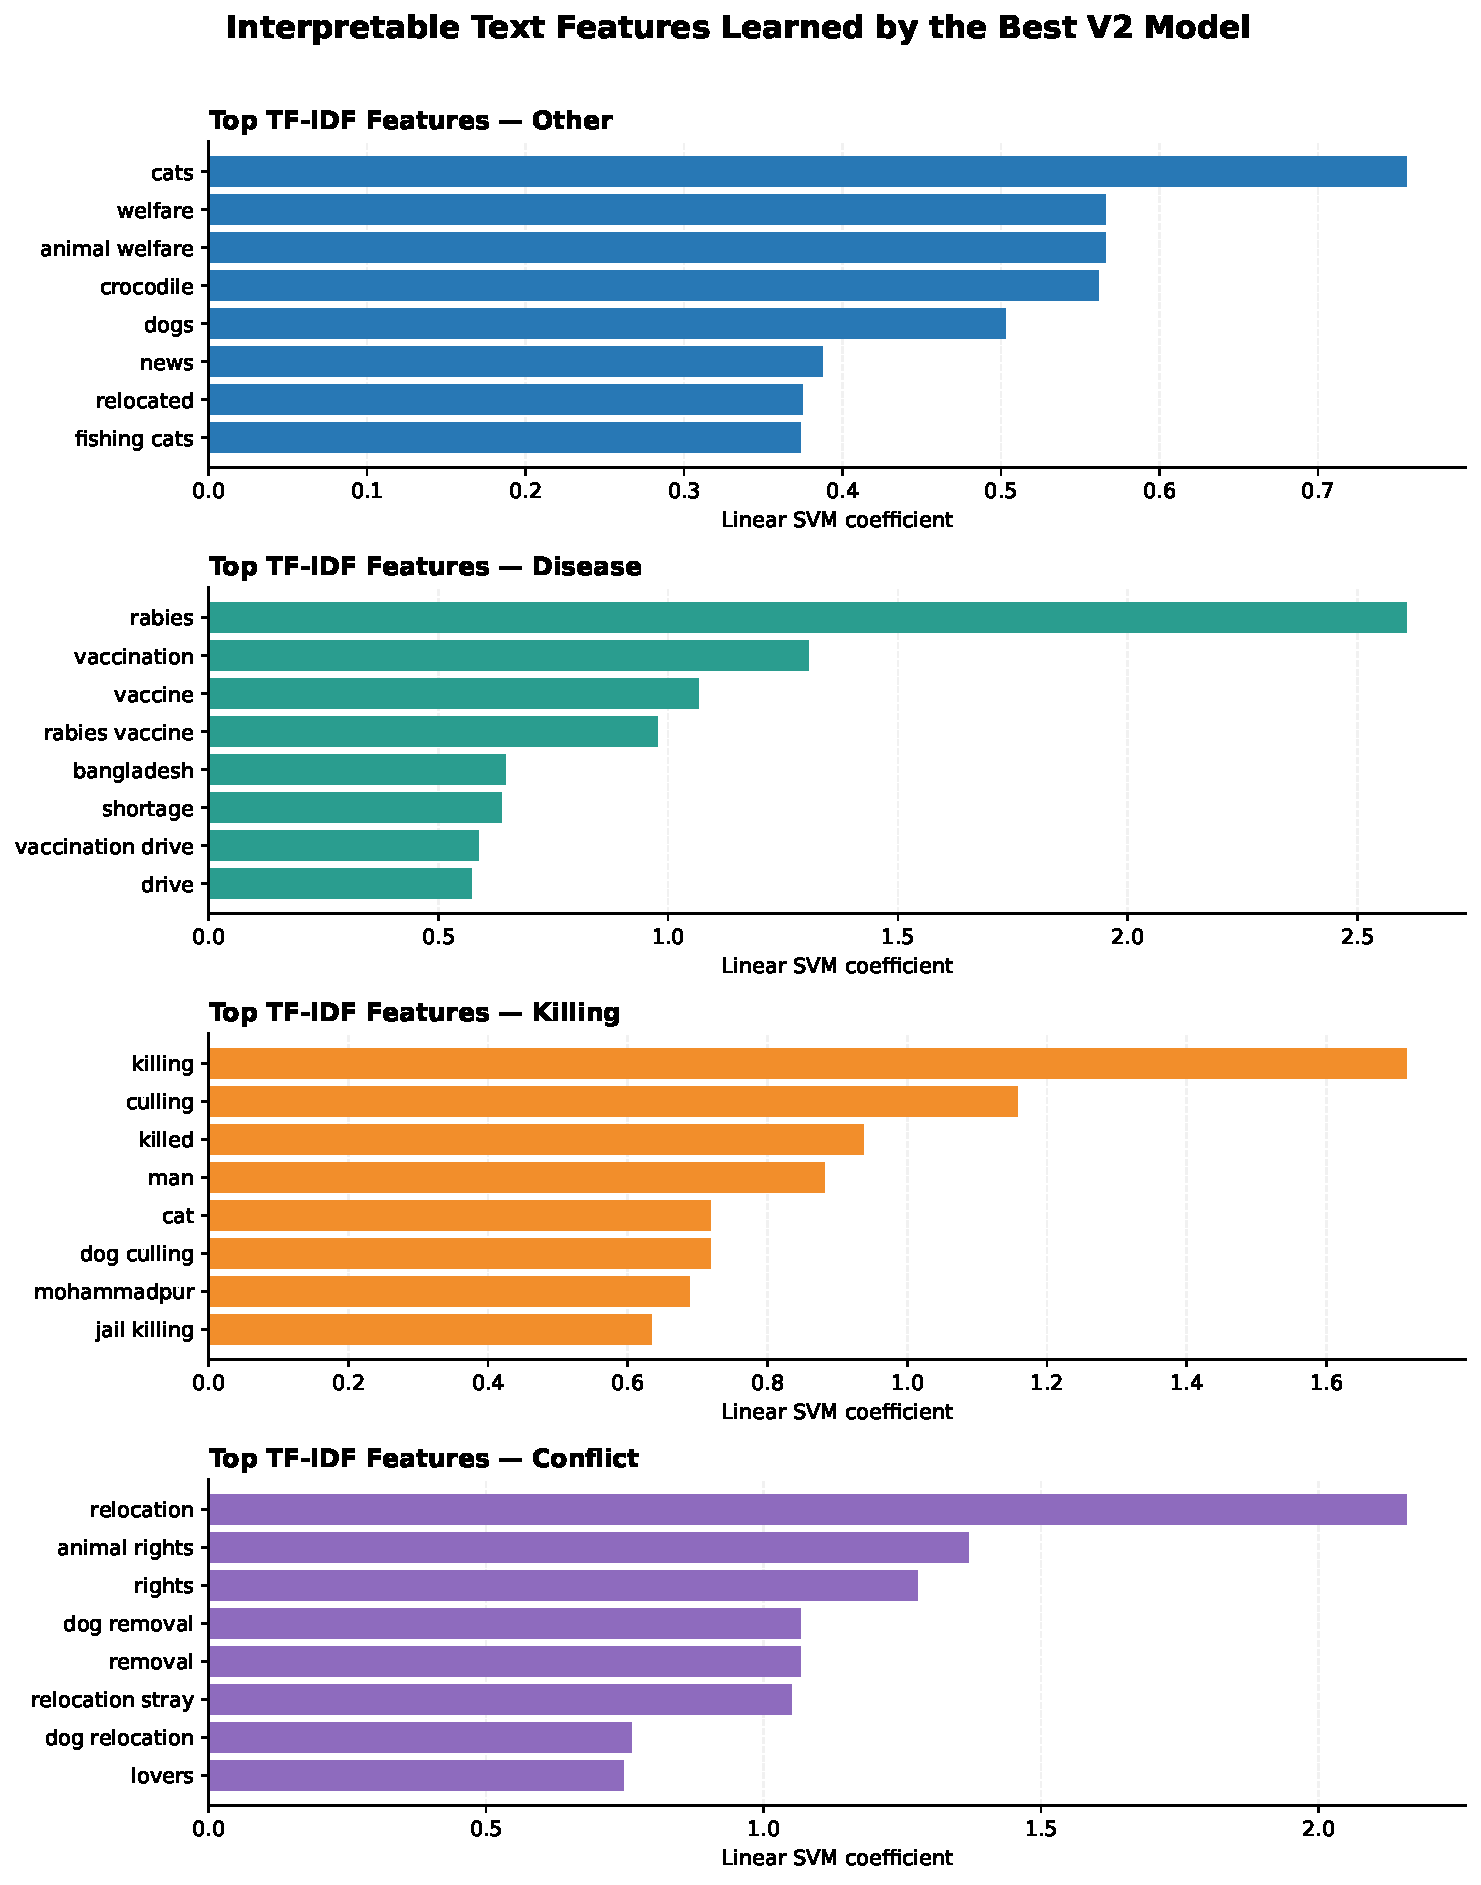
\includegraphics[width=0.90\textwidth]
    {final_top_features.pdf}
    \caption{Representative highest-weighted TF--IDF features for four incident
    categories identified by the selected Linear SVM model. Positive feature
    weights indicate terms that contributed more strongly to the corresponding
    class decision.}
    \label{fig:top_features}
\end{figure*}

The feature analysis is useful for two reasons. First, it allows inspection
of whether the classifier is learning terms that are reasonably connected
with the intended incident categories. Second, it can reveal undesirable
shortcuts, such as excessive dependence on a source name, location, or a
small number of highly specific keywords.

However, the feature weights should not be interpreted as causal explanations.
A high coefficient indicates that a feature contributes strongly to a
decision boundary learned from this corpus; it does not imply that the term
causes the underlying welfare event.

A further concern arises from the labeling procedure. Most training labels
were initially generated using domain-specific textual rules. Some of the
same lexical signals may therefore appear both in the weak-label construction
process and in the TF--IDF representation used by the classifier. This can
produce a degree of label-feature dependence and may make classification
performance appear stronger than it would be against a fully independent
expert-annotated dataset. The feature analysis consequently serves not only
as an explanation mechanism but also as a diagnostic tool for identifying
this potential source of leakage.

\FloatBarrier

% =========================================================
% XI. COMPARISON WITH THE EARLIER FRAMEWORK
% =========================================================

\section{Evolution from the Earlier Framework}

The present work is an extension of an earlier news-based stray-animal risk
assessment pipeline. The earlier version established the feasibility of
collecting online news records, assigning rule-based incident categories,
calculating a simple severity score, and visualizing the resulting patterns.
That version provided a useful proof of concept, but several limitations
became apparent during its implementation.

In particular, incident assignment relied primarily on predefined lexical
rules, textual context was limited, geographic information was inconsistent,
and the risk calculation was simplified in implementation. The earlier
framework also lacked a direct field-observation component.

V2 was therefore designed as a methodological extension rather than merely
an increase in dataset size.

\begin{table*}[!t]
\centering
\caption{Methodological Evolution from V1 to V2}
\label{tab:v1_v2}
\renewcommand{\arraystretch}{1.18}
\begin{tabular}{p{0.20\textwidth}p{0.34\textwidth}p{0.38\textwidth}}
\toprule
\textbf{Component} & \textbf{Earlier Framework (V1)} &
\textbf{Current Framework (V2)} \\
\midrule

News processing &
News scraping followed by basic cleaning and rule-based categorization. &
Expanded retrieval followed by content relevance filtering, Bangladesh-scope
refinement, and assisted review. \\

Incident analysis &
Incident categories assigned using deterministic textual rules. &
Eight-class supervised text classification using TF--IDF with Linear SVM,
Logistic Regression, and Complement Naive Bayes. \\

Model evaluation &
No comparative supervised incident-classification experiment. &
Stratified cross-validation with Accuracy, Macro Precision, Macro Recall,
Macro F1, and Weighted F1. \\

Risk assessment &
Simple rule-based severity assignment associated closely with incident type. &
Separate five-component SARI V2 heuristic with explicit 0--10 scoring and
documented thresholds. \\

Interpretability &
Primarily rule-level transparency. &
Inspection of learned Linear SVM TF--IDF feature weights in addition to
transparent SARI components. \\

Geographic handling &
Location information was frequently unavailable or inconsistent. &
Explicit Bangladesh-primary scope refinement; unsupported geographic hotspot
claims are avoided. \\

Field evidence &
Not incorporated. &
Structured pilot observations of 325 free-roaming animals across four Badda
localities. \\

Framework design &
Primarily news-oriented analytical pipeline. &
Dual-source architecture combining event-oriented news intelligence with
condition-oriented field intelligence. \\

\bottomrule
\end{tabular}
\end{table*}

The comparison demonstrates that the main advancement in V2 is not a single
classifier or visualization. The larger change is the restructuring of the
project into a more defensible analytical workflow in which data scope,
label quality, model evaluation, risk assessment, and field evidence are
treated as separate methodological problems.

% =========================================================
% XII. DISCUSSION AND PRACTICAL IMPLICATIONS
% =========================================================

\section{Discussion and Practical Implications}

The findings illustrate both the potential and the limitations of using
heterogeneous data for stray-animal welfare analysis in Bangladesh. The news
pipeline shows that publicly available reports can be transformed into a
structured incident corpus, while the field survey demonstrates that
important welfare indicators are often visible only through direct local
observation.

\subsection{Lessons from the News Intelligence Component}

One of the clearest findings from the news pipeline is the importance of data
refinement. Starting from 1,094 candidate records, only 690 remained after
content relevance filtering, and only 250 were classified as
Bangladesh-primary. Following assisted-review decisions, the final
machine-learning corpus contained 226 records.

This reduction is not simply data loss. It reflects an attempt to reduce
noise introduced by search retrieval, foreign reports, wildlife-related
content, and ambiguous uses of animal-related terminology. A larger but
poorly scoped dataset would have produced more observations while weakening
the connection between the analysis and the intended Bangladesh context.

The Linear SVM achieved the strongest overall balance among the evaluated
classifiers, with a Macro F1 of 0.6068 and Weighted F1 of 0.7517. These
results are encouraging for a proof-of-concept system, particularly given
the small corpus. At the same time, the failure to recover the Rescue class
and the weak recall for several rare categories demonstrate that the current
dataset is not sufficient for reliable automated classification across every
incident type.

\subsection{Lessons from SARI V2}

SARI V2 adds a different analytical perspective. Rather than attempting to
predict a weakly constructed risk label through another supervised model, it
uses transparent components to summarize the textual and contextual signals
associated with an incident.

The resulting scores were concentrated in the Low and Medium ranges, with no
record reaching the predefined High-risk threshold. This result is useful
precisely because the scoring thresholds were not changed after observing the
distribution. Adjusting the threshold merely to generate High-risk cases
would make the resulting visualization more dramatic but would weaken the
methodological consistency of the framework.

The current SARI V2 should therefore be viewed as a prototype prioritization
mechanism. Future validation against independently assessed welfare outcomes
would be necessary before assigning operational meaning to particular score
thresholds.

\subsection{Lessons from the Badda Pilot Survey}

The field survey reveals a different set of concerns. Among 325 observed
animals, only 9.85\% were recorded as vaccinated and 10.46\% as sterilized.
In addition, 28.62\% were recorded as either underweight/malnourished or
starved.

These results do not establish prevalence for Badda as a whole, and they
certainly do not represent Bangladesh nationally. Nevertheless, they
demonstrate the type of local information that structured welfare surveys can
produce. Such information can support practical planning for vaccination,
sterilization, feeding assistance, veterinary assessment, and repeat
surveying.

The location-specific results can also be used as prompts for further
investigation. For example, no vaccinated animals were observed within the
surveyed Dokkhin Badda sample, while no sterilized animals were recorded
within the surveyed Jheelpar sample. These findings should trigger additional
data collection rather than immediate area-wide conclusions.

\subsection{Potential Use in Welfare Operations}

A future operational version of the framework could support local animal
welfare groups, researchers, and relevant authorities through a shared
decision-support interface. Incoming news could be organized into incident
categories, while field teams could update structured animal observations
from selected localities.

The resulting system could help answer practical questions such as which
incident categories are appearing in the monitored media corpus, which
locations have low observed intervention coverage, where repeat surveys may
be useful, and which records deserve manual review.

Human review would remain important. The framework is intended to organize
evidence and support prioritization, not to automate veterinary diagnosis,
legal judgment, or intervention decisions.

% =========================================================
% XIII. LIMITATIONS
% =========================================================

\section{Limitations}

Several limitations should be considered when interpreting the results.

First, the news dataset is based on Google News RSS retrieval and therefore
does not represent a complete census of stray-animal incidents in Bangladesh.
Search ranking, indexing, source availability, query design, and media
attention all influence which events appear in the collected corpus.

Second, full article text was not consistently available. The analysis relies
primarily on headlines and available RSS descriptions. This restricts the
amount of contextual information available for relevance filtering, incident
classification, geographic interpretation, and SARI V2 scoring.

Third, the incident labels are not a fully independent expert-annotated gold
standard. They were generated through weak supervision and partially checked
through assisted review. Although the reviewed retained subset showed 90.0\%
agreement with the initial suggested labels, this value is not an estimate of
model accuracy or expert annotation quality.

Fourth, lexical rules used during weak-label construction can overlap with
features later learned by the TF--IDF classifier. This creates a potential
source of label-feature dependence. Consequently, the reported
cross-validation scores may overestimate performance relative to evaluation
against independently annotated unseen data.

Fifth, the final machine-learning corpus is small and strongly imbalanced.
Poisoning contains only three records and Rescue only two. Metrics for these
classes are therefore unstable, and the selected classifier should not be
considered production-ready.

Sixth, SARI V2 is a heuristic index. Its component weights and Low, Medium,
and High thresholds were designed for interpretability but have not been
externally calibrated against clinical, epidemiological, or independently
assessed welfare outcomes.

Seventh, geographic analysis of the news corpus remains limited. Reliable
coordinates were not available for the majority of records, so techniques
such as DBSCAN or HDBSCAN hotspot detection were not applied. Introducing
such methods without reliable location data would create artificial
precision.

Eighth, the Badda field survey is a localized pilot sample. Survey coverage
is uneven across the four localities, with substantially more observations
from Uttar Badda. The sample was not designed to estimate population-level
prevalence, and the observed health categories were not confirmed through
veterinary examinations.

Finally, although photographs were collected during the field survey, they
were not used as verified labels for computer-vision training or clinical
assessment. The current study therefore makes no image-based diagnostic
claims.

% =========================================================
% XIV. FUTURE WORK
% =========================================================

\section{Future Work}

The next stage of the project should focus primarily on improving evidence
quality rather than simply increasing model complexity.

A larger independently annotated news corpus would allow more reliable model
evaluation and provide sufficient examples for rare categories such as
Poisoning, Rescue, and Human-Animal Conflict. Annotation by multiple human
reviewers would also make it possible to measure inter-annotator agreement
and construct a stronger evaluation benchmark.

The news pipeline can be extended from headlines and RSS descriptions to
full-text article processing where legally and technically available. Richer
text would support more accurate event extraction, location identification,
entity recognition, and contextual classification.

Geographic analysis is another important direction. If reliable coordinates
or consistently normalized location fields become available, the framework
could support spatial clustering and hotspot analysis. Methods such as DBSCAN
or HDBSCAN should be introduced only after the geographic evidence is
sufficiently complete and accurate.

SARI V2 also requires further validation. Future work could involve animal
welfare professionals or veterinarians in reviewing representative incidents
and assessing whether the component weights and thresholds correspond to
meaningful intervention priorities.

The field component should be expanded beyond Badda using a more systematic
sampling strategy. Repeated surveys across additional neighborhoods and
districts would allow the framework to distinguish persistent conditions from
short-term observations and would improve the geographic relevance of the
field intelligence.

Survey photographs could eventually support computer-vision research, but
this would require explicit image-label definitions, quality control,
privacy safeguards, and substantially more verified examples. Image-based
health assessment should not be attempted solely from the existing
unvalidated photographs.

Finally, the two evidence streams could be exposed through an interactive
dashboard with appropriate uncertainty indicators. Such a platform could
support incident review, survey monitoring, intervention tracking, and
periodic updates while retaining human oversight.

% =========================================================
% XV. CONCLUSION
% =========================================================

\section{Conclusion}

This study presents a machine learning-driven stray-animal welfare
intelligence framework designed for the Bangladesh context. The work extends
an earlier news-based risk-assessment pipeline by introducing stricter data
refinement, supervised incident classification, an interpretable SARI V2
risk index, and a localized field-intelligence component.

The news pipeline expanded to 1,094 candidate records, of which 690 remained
after relevance filtering, 250 were identified as Bangladesh-primary, and
226 formed the final machine-learning corpus after assisted-review decisions.
Among three evaluated classifiers, Linear SVM produced the strongest Macro
F1 score of 0.6068 and a Weighted F1 of 0.7517.

SARI V2 provided a separate heuristic assessment of textual and contextual
severity. The mean score was 1.550, with 191 records categorized as Low and
35 as Medium; no record crossed the predefined High-risk threshold.

The field component added direct observations of 325 free-roaming animals
from four localities in Badda, Dhaka. Within this pilot sample, 9.85\% were
recorded as vaccinated, 10.46\% as sterilized, and 28.62\% showed an observed
nutritional health concern.

The main contribution of the study lies in connecting these two perspectives
without treating them as equivalent datasets. News intelligence provides a
view of reported events, while field intelligence provides a view of observed
local conditions. Their evidence-level integration creates a more complete
foundation for welfare-oriented decision support than either source could
provide independently.

The framework remains a proof of concept rather than a national surveillance
or clinical decision system. Nevertheless, it establishes a reproducible
foundation that can be strengthened through expert annotation, broader field
coverage, improved geographic information, validated risk scoring, and
continued data collection.


\bibliographystyle{IEEEtran}
\bibliography{references_v2}
\end{document}